\documentclass{article}
\usepackage[left=1in,right=1in,top=1in, bottom=1in]{geometry}
\usepackage{physics}
\usepackage{graphicx}
\usepackage{caption}
\usepackage{amsmath}
\usepackage{bm}
\usepackage{authblk}
\usepackage{framed}
\usepackage{empheq}
\usepackage{amsfonts}
\usepackage{esint}
\usepackage[makeroom]{cancel}
\usepackage{dsfont}
\usepackage{centernot}
\usepackage{mathtools}
\usepackage{bigints}
\usepackage{amsthm}
\theoremstyle{definition}
\newtheorem{defn}{Definition}[section]
\newtheorem{prop}{Proposition}[section]
\newtheorem{rmk}{Remark}[section]
\newtheorem{thm}{Theorem}[section]
\newtheorem{cor}{Corollary}[section]
\newtheorem{exmp}{Example}[section]
\newtheorem{prob}{Problem}[section]
\newtheorem{sln}{Solution}[section]
\newtheorem*{prob*}{Problem}
\newtheorem{exer}{Exercise}[section]
\newtheorem*{exer*}{Exercise}
\newtheorem*{sln*}{Solution}
\usepackage{empheq}
\usepackage{hyperref}
\usepackage{tensor}
\usepackage{xcolor}
\hypersetup{
	colorlinks,
	linkcolor={black!50!black},
	citecolor={blue!50!black},
	urlcolor={blue!80!black}
}


\newcommand*\widefbox[1]{\fbox{\hspace{2em}#1\hspace{2em}}}

\newcommand{\p}{\partial}
\newcommand{\R}{\mathbb{R}}
\newcommand{\C}{\mathbb{C}}
\newcommand{\lag}{\mathcal{L}}
\newcommand{\nn}{\nonumber}
\newcommand{\ham}{\mathcal{H}}
\newcommand{\M}{\mathcal{M}}
\newcommand{\I}{\mathcal{I}}
\newcommand{\K}{\mathcal{K}}
\newcommand{\F}{\mathcal{F}}
\newcommand{\w}{\omega}
\newcommand{\lam}{\lambda}
\newcommand{\al}{\alpha}
\newcommand{\be}{\beta}
\newcommand{\x}{\xi}

\newcommand{\G}{\mathcal{G}}

\newcommand{\f}[2]{\frac{#1}{#2}}

\newcommand{\ift}{\infty}

\newcommand{\lp}{\left(}
\newcommand{\rp}{\right)}

\newcommand{\lb}{\left[}
\newcommand{\rb}{\right]}

\newcommand{\lc}{\left\{}
\newcommand{\rc}{\right\}}


\newcommand{\V}{\mathbf{V}}
\newcommand{\U}{\mathcal{U}}
\newcommand{\Id}{\mathcal{I}}
\newcommand{\D}{\mathcal{D}}
\newcommand{\Z}{\mathcal{Z}}

%\setcounter{chapter}{-1}


%\makeatletter
%\renewcommand{\@chapapp}{Part}
%\renewcommand\thechapter{$\bf{\ket{\arabic{chapter}}}$}
%\renewcommand\thesection{$\bf{\ket{\arabic{section}}}$}
%\renewcommand\thesubsection{$\bf{\ket{\arabic{subsection}}}$}
%\renewcommand\thesubsubsection{$\bf{\ket{\arabic{subsubsection}}}$}
%\makeatother

%\usepackage{newpxtext,newpxmath}

\usepackage{subfig}
\usepackage{listings}
\captionsetup[lstlisting]{margin=0cm,format=hang,font=small,format=plain,labelfont={bf,up},textfont={it}}
\renewcommand*{\lstlistingname}{Code \textcolor{violet}{\textsl{Mathematica}}}
\definecolor{gris245}{RGB}{245,245,245}
\definecolor{olive}{RGB}{50,140,50}
\definecolor{brun}{RGB}{175,100,80}
\lstset{
	tabsize=4,
	frame=single,
	language=mathematica,
	basicstyle=\scriptsize\ttfamily,
	keywordstyle=\color{black},
	backgroundcolor=\color{gris245},
	commentstyle=\color{gray},
	showstringspaces=false,
	emph={
		r1,
		r2,
		epsilon,epsilon_,
		Newton,Newton_
	},emphstyle={\color{olive}},
	emph={[2]
		L,
		CouleurCourbe,
		PotentielEffectif,
		IdCourbe,
		Courbe
	},emphstyle={[2]\color{blue}},
	emph={[3]r,r_,n,n_},emphstyle={[3]\color{magenta}}
}


\begin{document}




\begin{center}
	\textbf{\Large{Defining and Evaluating $H^t_\Pi(\vec{x})$}}\\
	{Huan Q. Bui, Evan Randles}\\
	\today\\
\end{center}


\tableofcontents

\newpage



\section{Useful Definitions \& Theorems}

\begin{defn}
(Riemann-integrability) Here's a suggestive definition of Riemann-integrability. A bounded function $f: I \to \mathbb{R}$ is said to be Riemann-integrable whenever
\begin{align*}
    \inf_P U(f,P) = \overline{\int_I}f = \underline{\int_I} f = \sup_P L(f,P)
\end{align*}
where $P$ is any partition of $I$, and $U,L$ denote the upper and lower sums, respectively. 
\end{defn}

 
\begin{defn}
(Rectifiable set) Let $S \subset \mathbb{R}^n$. If the constant function $1$ is \textit{Riemann-integrable} over $S$ then $S$ is said to be \textit{rectifiable}. The value of this integral is defined to be the \textit{volume} of $S$:
\begin{align*}
    \text{vol}\,S = \int_S 1.
\end{align*}
\end{defn}


\begin{thm}
    $S \subset \mathbb{R}^n$ is rectifiable iff $S$ is bounded and $\text{Bd}\,S$ has measure zero.
\end{thm}

\begin{thm}
    Some useful properties:
    \begin{enumerate}
        \item $S$ rectifiable $\implies \text{Int}\,S$ is rectifiable and $\text{vol}\,S = \text{vol}\,\text{Int}\,S$.
        \item $S$ is rectifiable and $f:S\to \mathbb{R}$ is a bounded continuous function $\implies f$ is Riemann-integrable over $S$. 
    \end{enumerate}
\end{thm}



\begin{defn}
    (Extended Integral) Let $A\overset{\text{open}}{\subset} \mathbb{R}^n$ and $f:A \xrightarrow{\text{cont., non-neg. on } A } \mathbb{R}$ be given. Then the extended integral of $f$ over $A$ is defined to be
    \begin{align*}
        \int_A f = \sup_D \int_D f
    \end{align*}
    where $D$ ranges over all compact rectifiable subsets of $A$. When the supremum exists, we say $f$ is integrable over $A$ in the extended sense. If $f$ is not necessarily nonnegative on $A$, we say $f$ is integral over $A$ in the extended sense if both 
    \begin{align*}
        f_+ \coloneqq \max\{ f(x),0 \} \text{ and } f_- \coloneqq \max\{ -f(x),0 \}
    \end{align*}
     are extended-integrable over $A$. In this case, the extended integral of $f$ over $A$ is:
    \begin{align*}
        \int_A f = \int_A f_+ - \int f_-.
    \end{align*}
\end{defn}






\begin{thm}
    Let $A \overset{\text{open}}{\subset} \mathbb{R}^n$ be given. Then there exists a sequence $C_1,C_2,\dots$ of compact rectifiable subsets of $A$ such that $A = \bigcup_i U_i$ and $C_N \subset \text{Int}\,C_{N+1}$ for each $N$. 
\end{thm}




\begin{thm}
    Let $A\overset{\text{open}}{\subset} \mathbb{R}^n$ and $f: A \xrightarrow{\text{cont.}} \mathbb{R}$. Choose a sequence $C_N$ of compact rectifiable subsets of $A$ such that $A = \bigcup_i U_i$ and $C_N \subset \text{Int}\,C_{N+1}$ for each $N$. Then $f$ is extended-integrable over $A$ iff the sequence $\int_{C_N}\abs{f}$ is bounded. In this case, 
    \begin{align*}
        \int_A f = \lim\limits_{N\to \infty} \int_{C_N} f.
    \end{align*}
\end{thm}



\begin{thm}
    $f$ is (extended) integrable over $A$ $\iff$ $\abs{f}$ is (extended) integrable over $A$. 
\end{thm}


\begin{thm}
    Let $A \overset{\text{bdd, open}}{\subset} \mathbb{R}^n$ and $f: A \xrightarrow{\text{bdd, cont.}} \mathbb{R}$ be given. Then the extended integral $\int_A f$ exists. If the ordinary integral $\int_A f$ also exists, then these two integrals are equal.
\end{thm}


\begin{cor}
    Let $S \overset{\text{bdd}}{\subset} \mathbb{R}^n$ and $f: S \xrightarrow{\text{bdd, cont}}$ be given. If $f$ is ordinary-integrable over $S$ then 
    \begin{align*}
        \text{(ord.)} \int_S f = \text{(ext.)} \int_{\text{Int}\,S} f.
    \end{align*}
\end{cor}




\begin{thm}
    Let $A \overset{\text{open}}{\subset} \mathbb{R}^n$, $f: A \xrightarrow{\text{cont.}} \mathbb{R}$ be given. Let $U_1 \subset U_2 \subset \dots$ be open sets such that $A = \bigcup_i U_i$. Then $\int_A f$ exists iff the sequence $\int_{U_n}\abs{f}$ exists and is bounded. In this case,
    \begin{align*}
        \int_A f = \lim\limits_{N\to \infty}\int_{U_N}f.
    \end{align*}
\end{thm}












\newpage




\section{Small-Tail Condition}

\begin{defn}
Let $f\in L^1_{\mbox{\footnotesize loc}}(\mathbb{R}^d)$. We say that $f$ satisfies the small tail condition if, for all $\epsilon>0$, there exists a bounded domain $\mathcal{O}\subseteq\mathbb{R}^d$ such that, for every connected compact rectifiable set $C\subseteq \mathbb{R}^d\setminus\mathcal{O}$, 
\begin{equation*}
\left|\int_C f\right|<\epsilon.
\end{equation*}
\end{defn}

\textcolor{red}{The space $L^1_{\text{loc}}(\mathbb{R}^d)$ (the locally integrable functions) is the space of Lebesgue measurable functions for which, given any compact set $K\subseteq \mathbb{R}^d$, the product $f(x)\chi_{K}(x)$ is absolutely (Lebesgue) integrable; here, $\chi_K$ is the ``characteristic" or ``indicator" function on the set $K$. I believe this is the correct generality for us -- though you should not worry much about the details (though I'm happy to cover them) concerning Lebesgue integrability. What you really need to know, for now, is that if $f$ is Riemann-integrable on a compact set $K$, then it is Lebesgue integrable on $K$ and the two integrals agree. In particular, if a function $f:\mathbb{R}^d\to\mathbb{C}$ is continuous, it is Riemann-integrable on any compact set $K$ and therefore it is locally integrable.}

\begin{defn}
An approximating sequence of $\mathbb{R}^d$, or simply an approximating sequence, is a collection $\{C_n\}_{n\in\mathbb{N}}$ of \textcolor{red}{simply} connected, compact, and rectifiable sets which are nested in the sense that $C_n\subseteq \mbox{Int}(C_{n+1})$ for each $n\in\mathbb{N}$ and whose union is all of $\mathbb{R}^d$, i.e., $\bigcup_{n=1}^\infty C_n=\mathbb{R}^d$.
\end{defn}
Questions/Comment:

\begin{enumerate}
\item Does this depend on being a domain or a general open set?
\item We should use the word integrable somewhere. 
\item Can we prove: 
\begin{thm}
Suppose that $f\in L^1_{\text{loc}}(\mathbb{R}^d)$ satisfies the small tail condition. Then, given any approximating sequence $\{C_n\}$ of $\mathbb{R}^n$
\begin{equation*}
I=\lim_{n\to\infty}\int_{C_n} f
\end{equation*}
exists. Further, this limit is independent of the approximating sequence chosen.
\end{thm}

\begin{defn}
Let $f\in L^1_{\mbox{\tiny}}(\mathbb{R}^d)$ satisfying the small tail condition. The improper Lebesgue integral of $f$ is the number
\begin{equation*}
\int_{\mathbb{R}^d} f= I=\lim_{n\to\infty}\int_{C_n}f(x)\,dx
\end{equation*}
where $\{C_n\}$ is an approximating sequence of $\mathbb{R}^d$.
\end{defn}

\item Can we show that all improperly integrable functions in the sense of Munkres satisfy the small tail condition and, if so, does his integral coincide with ours?
\item Is our integral linear?
\item Does $f(\xi)=\cos(\xi^3)$ satisfy the small tail condition on $\mathbb{R}^d=\mathbb{R}$? -- should be a consequence of van der Corput. 
\end{enumerate}




\hrule


$\,$\\


\noindent \texttt{Mar 28, 2020:} \\




\begin{exmp}
Consider $f: \mathbb{R} \xrightarrow{\text{cont.}} \mathbb{R}$ the Cauchy distribution given by
\begin{align*}
    f(x) = \f{1}{\pi(1+x^2)}.
\end{align*}
Since $f$ is a probability distribution, 
\begin{align*}
    1 = \int^\infty_{-\infty} f \coloneqq \text{P.V.} \int^\infty_{-\infty}f =\lim\limits_{t\to\infty}\int^t_{-t}f  
\end{align*}
where $\text{P.V.}$ denotes ``Cauchy principal value.'' The Cauchy distribution is known to have a ``heavy-tail,'' so heavy that its expectation value and variance are not defined. \\ 

However, \underline{$f$ \textit{does} satisfy the small-tail condition defined above}. Let $\epsilon > 0$ be given. Let the domain $\mathcal{O}$ be of the form $(-t,t)$ where $t$ is some positive number. Provided $\epsilon$, if we can always find a value of $t$ such that $\forall C \overset{\text{com.rect.}}{\subseteq} \mathbb{R}\setminus \mathcal{O}$, $\abs{\int_C f} < \epsilon$ then we're done. This is just a matter of finding $t$ such that ${\int^t_{-t}f}$ is sufficiently large. We have
\begin{align*}
    \int^t_{-t}f(x)\,dx = \f{2\arctan(t)}{\pi}.
\end{align*}
$\arctan(t)$ is a continuous and increasing function on $\mathbb{R}$ with range $[-\pi/2,\pi/2]$. By the Intermediate Value Theorem, $\exists t' \geq 0$ such that
\begin{align*}
\f{2\arctan(t')}{\pi} > 1-\epsilon \iff \abs{\int_\mathbb{R} f - \int_\mathcal{O}f} = \abs{\int_{\mathbb{R}\setminus\mathcal{O}}f} < \epsilon
\end{align*}
Since $f$ is nonnegative, for every compact rectifiable $C \subseteq \mathbb{R}\setminus\mathcal{O}$, $\int_C f \leq \int_\mathcal{O}f$. This means $\mathcal{O} = (-t',t')$ guarantees $\abs{\int_C f} < \epsilon$ for every $C \overset{\text{com.rect.}}{\subseteq} \mathbb{R}\setminus \mathcal{O}$. \qed\\






\noindent \textbf{Now we address Question 3:} Provided that $f$, the Cauchy pdf, satisfies the  small-tail condition, is it true that given any sequence of nested compact rectifiable sets $\{ C_n\}$,
\begin{align*}
    I = \lim\limits_{n\to \infty} \int_{C_n}f
\end{align*}
exists \textit{and} is independent of the choice of $\{C_n\}$? \\



\textit{Counter-example:} I will show that even though $f$ satisfies the small-tail condition, $I$ depends on the choice of $\{C_n\}$. First, consider $\{C_n\}$ where each $C_n$ has the form $(-n,n)$. As we have seen before,
\begin{align*}
    \int_{C_n}f = \frac{2\arctan(n)}{\pi}.
\end{align*}
In this case the $C_n$'s form a nested sequence of compact rectifiable subsets of $\mathbb{R}$ and 
\begin{align*}
    \lim_{n\to\infty}\int_{C_n}f =1.    
\end{align*}
However, consider now $\{C_n\}$ with $C_n = (e^{-n} - 1, n)$. Once again, since $n\geq 0$, the $C_n$'s form a nested sequence of subsets, but
\begin{align*}
    \lim_{n\to \infty}\int_{C_n}f = \frac{3}{4} \neq 1.
\end{align*}
This means we \underline{cannot} prove the claim made in item 3. At worst, $\bigcup_i U_i = \mathbb{R}$ to make this work.


\end{exmp}

\begin{exmp}
Here we show that $f(\xi)=\cos(\xi^3)$ does not satisfy the small tail condition as it stands.

Observe that $f(\xi)\geq 0$ whenever $\pi(2k-1)\leq \xi^3\leq \pi(2k+1)$ when $k$ is an integer. Correspondingly, $f$ is non-negative exactly on the set
\begin{equation*}
P=\bigcup_{k\in\mathbb{Z}}P_k. 
\end{equation*}
where $P_k=[(\pi(2k-1))^{1/3},(\pi(2k+1)^{1/3}]$ for each $k\in\mathbb{Z}$.
Noting that the graph of cosine is convex between any two consecutive zeros, by placing a triangle under the graph of cosine between each two consecutive zeros with ``upper'' vertex at the maximum of $1$, we obtain the estimate
\begin{equation*}
\int_{P_k}f(\xi)\,d\xi\geq \frac{1}{2}\left((\pi(2k+1))^{1/3}-(\pi(2k-1))^{1/3}\right)
\end{equation*}
for each $k\in\mathbb{Z}$. I believe this can easily be verified by L'Hopital's rule, the lower bound above is itself above $\pi^{1/3}/2k\geq 1/2k $ for integers $k>15$. Correspondingly, we have that
\begin{equation*}
\int_{P_k}f(\xi)\,d\xi>\frac{1}{2k}
\end{equation*}
for all $k\in\mathbb{Z}$ such that $k\geq 15$. As the Harmonic series is divergent, we have that
\begin{equation*}
\sum_{k=15}^\infty \int_{P_k}f(\xi)\,d\xi=\infty.
\end{equation*}
Okay, now take $\epsilon=1$ and let $\mathcal{O}$ be any domain (\textcolor{blue}{which is bounded}). Since $\mathcal{O}$ is bounded, there is some integer $K\geq 15$ such that, $\bigcup_{k=K}^\infty P_k\subseteq \mathbb{R}\setminus\mathcal{O}$. As convergence of non-negative series is determined by tails, we have
\begin{equation*}
\sum_{k=K}^\infty \int_{P_k}f(\xi)\,d\xi=\infty
\end{equation*}
and, in particular, there must be some $M\geq K$ for which
\begin{equation*}
\sum_{k=K}^M\int_{P_k}f(\xi)\,d\xi\geq 1. 
\end{equation*}
Consider now $C=\bigcup_{k=K}^{k=M}P_k$, we have that
\begin{equation*}
\left|\int_C f(\xi)\,d\xi\right|=\int_Cf(\xi)\,d\xi=\sum_{k=K}^M\int_{P_k}f(\xi)\,d\xi\ge 1=\epsilon.
\end{equation*}
Upon noting that $C$ is a finite union of (disjoint) rectifiable compact intervals, we conclude that $C$ is also compact and rectifiable and the assertion is proven.\qed
\end{exmp}











\begin{framed}

\textcolor{red}{\texttt{Mar 28, 2020 discussion:}}\\

From the above examples we add the ``connectedness'' condition to compact rectifiable sets $C$ in the small-tail condition and the theorem about the independence of $\{ C_n \}$.\\

\underline{To prove:} If $f$ satisfies the small tail condition, then given any nested connected compact rectifiable sets $\{C_n\}$ such that $\bigcup C_n = \mathbb{R}^d$, the limit $\lim\limits_{n\to\infty}\int_{C_n}f$ exists and is independent of the choice of $\{ C_n \}$. \\

\begin{proof}
Let $f$ be given such that $f$ satisfies the small tail condition. Let $\{C_n\}$ be such a sequence of nested sets. We want to show $\{ I_n \}$ is Cauchy (i.e., is convergent), where
\begin{align*}
    I_n = \int_{C_n}f.
\end{align*}

Wait... something's missing here

\end{proof}



Okay, so I think you will have already established that $I$ exists for a given sequence $\{C_n\}$ (so a little more work above). Ah\\


I'm trying to show $I$ exists first, which I'm having trouble with because I don't think the argument works for \textit{any} $\{C_n\}$. $f$ satisfying STC has to come in at some point, but STC says there exists a domain $O$ such that so long as the sets $C$ are in $\mathbb{R}^d\setminus \mathcal{O}$, $\abs{\int_C f}$ is small. This, in a way, says that I can't just pick any sequence $\{C_n \}$ to use STC.

So, I think you start how you started with an arbitrary (but fixed) sequence $\{C_n\}$. This sequence will define the set $\mathcal{O}$ for any $\epsilon$ desired, I think.

Let $f\in L^1_loc$ satisfy the STC and let $\{C_n\}$ be an approximating sequence of $\mathbb{R}^d$. Let $\epsilon>0$ and let $\mathcal{O}$ be a bounded domain for which $\left|\int_C f\right|<\epsilon$ for any connected compact rectifiable set $C\in \mathbb{R}^d\setminus \mathcal{O}$.

I claim that there is an $N\in\mathbb{N}$ for which $\mathcal{O}\subseteq C_N$. To see this, by the Heine-Borel theorem, the closure of $\mathcal{O}$, $K=\overline{\mathcal{O}}$ is a compact set. Also, given that $\{C_n\}$ is an approximating sequence,  it is true that $\{\mbox{Int}(C_n)\}$ forms an open cover of $K$. By extracting a finite subcover, the fact that the sequence $\{C_n\}$ is nested, implies that the maximal index for this finite subcover, $N$, has
\begin{equation*}
\mathcal{O}\subseteq K\subseteq \mbox{Int}(C_N)\subseteq C_N,
\end{equation*}
which proves the claim.

Okay, now for any $n\geq m\geq N$, we have
\begin{equation*}
|I_n-I_m|=\left|\int_{C_n\setminus C_m}f\right|=\left|\int_{\overline{C_n\setminus C_m}} f\right|.
\end{equation*}
We note, however, that $\overline{C_n\setminus C_m}$ is (and we should check the connected thing rigorously) is a compact rectifiable connected subset of $\mathbb{R}^d$ and, because $\mathcal{O}\subseteq C_N\subseteq C_m$, it follows that $C_n\setminus C_n\subseteq \mathbb{R}^d\setminus \mathcal{O}$ and hence 
\begin{equation*}
|I_n-I_m|=\left|\int_{\overline{C_n\setminus C_m}} f\right|<\epsilon.
\end{equation*}


Yes, okay I got the idea at $\mathcal{O} \subseteq C_N$. Yes I got it.\\

Great! Good good good! This is great news then. Do you think that you can prove the Independence of sequence part?\\

I'll try. I haven't thought about it yet.\\

Okay, great. I'm going to give up for tonight. But, I'm pretty sure we're on to something. I'll add three comments/questions here:

\begin{enumerate}
\item More than the improper Riemann-integrability condition of Munkres, I know how to prove that if $f$ is Lebesgue integrable (i.e., if $f\in L^1(\mathbb{R}^d)$), then it automatically satisfies the small tail condition. This is actually a very fast consequence of the Dominated Convergence Theorem. Moreover, in this case, our definition of the integral agrees with that of Lebesgue. So this is great!

\item We should give a rigorous argument that $f(\xi)=\cos(\xi^3)$ satisfies the small tail condition. 

\item We should compare our definition against that gotten from distribution theory. I know you have already seen a little distribution theory from Physics. There is a result that says that any locally integrable function defines a distribution. I'm wondering if our integral is meaningful (or already understood) as some limit of distributions. I'm not sure how this would work, but I'm guessing there is something here. 

\item Okay, I'm done. Fantastic, you're doing a great job. 

\item Great, tty then.

Okay, I'll write something and think about the independence statement while doing my taxes :) \\

Thanks. I'll talk to you on Tuesday.

\end{enumerate}
\end{framed}














\noindent \texttt{Mar 31, 2020:} \\

\noindent \underline{To prove:} (Existence of the limit $I$) If $f$ satisfies the small tail condition, then given any sequence of nested \textcolor{red}{simply} connected compact rectifiable sets $\{C_n\}$ such that $\bigcup C_n = \mathbb{R}^d$, the limit $\lim\limits_{n\to\infty}\int_{C_n}f$ exists and is independent of the choice of $\{ C_n \}$. \\

\begin{proof}
Let $f$ be given such that $f$ satisfies the STC. Let $\{C_n\}$ be an approximating sequence. We want to show $\{ I_n \}$ is Cauchy (i.e., is convergent), where
\begin{align*}
    I_n = \int_{C_n}f.
\end{align*}
Let $ \epsilon > 0$ be given. Since $f$ satisfies the STC, there exists a bounded domain $\mathcal{O}$ for which $\abs{\int_C f} < \epsilon$ for any connected compact rectifiable set $C \subseteq \mathbb{R}^d\setminus\mathcal{O}$. By Heine-Borel, $\overline{\mathcal{O}}$ is compact. Further, since $\{ C_n \}$ is an approximating sequence, $\{ \mbox{Int}\,C_n \}$ forms an open cover of $\verline{\mathcal{O}}$. $\overline{\mathcal{O}}$ is compact so $\{ \text{Int}\,C_n\}$ contains a finite subcover. Now, because $\{C_n \}$ is nested, there is an $N\in\mathbb{N}$ such that 
\begin{align*}
    \mathcal{O} \subseteq \overline{\mathcal{O}} \subseteq \text{Int}\,C_N \subseteq C_N.
\end{align*}
It follows that for any $n\geq m\geq N$,
\begin{align*}
    \abs{I_n - I_m} = \abs{\int_{C_n\setminus C_m} f} = \abs{\int_{\overline{C_n\setminus C_m}} f}
\end{align*}
and $C_n\setminus C_m \subseteq \mathbb{R}^d\setminus \mathcal{O}$. Since $C_n\setminus C_m$ is connected (lemma), $\overline{C_n\setminus C_m}$ is a connected compact and rectifiable subset of $\mathbb{R}^d\setminus \mathcal{O}$. It follows from STC that 
\begin{align*}
    \abs{I_n - I_m} = \abs{\int_{C_n\setminus C_m} f} = \abs{\int_{\overline{C_n\setminus C_m}} f} < \epsilon.
\end{align*}
 




%We claim that $\overline{C_n\setminus C_m}$ is a connected compact rectifiable subset of $\mathbb{R}^d$. To this end we only need to check for connectedness. Suppose there exist disjoint nonempty open sets $\mathcal{U}$ and $\mathcal{V}$ such that $\mathcal{U}\cup \mathcal{V} = \overline{C_n\setminus C_m}$.  

\end{proof}









\noindent \underline{To prove}: (Independence of choice of $\{C_n\}$) If $f$ satisfies STC, then given any sequence of nested \textcolor{red}{simply} connected compact rectifiable sets $\{C_n \}$ such that $\bigcup U_n = \mathbb{R}^d$, $\lim_{n\to \infty}\int_{C_n} f$ exists (proved) and is independent of the choice of $\{C_n \}$

\begin{proof}
    Let approximating sequences $\{C_n \}$ and $\{ B_n \}$ be given and let 
    \begin{align*}
        I = \lim_{n\to\infty} \int_{C_n}f.
    \end{align*}
    We have shown $I$ exists. Let $\epsilon > 0$ be given. Then since $f$ satisfies STC, there exists a bounded domain $\mathcal{O}$ such that $\abs{\int_{D} f} < \epsilon/2$ for any connected compact rectifiable $D \subseteq \mathbb{R}^d\setminus \mathcal{O}$. We have argued that there exists $N \in \mathbb{N}$ such that
    \begin{align*}
        \mathcal{O} \subseteq \overline{\mathcal{O}} \subseteq \mbox{Int}\,C_N \subseteq C_N.
    \end{align*}
    Further, since $I$ exists, there exists $M\in \mathbb{N}$ such that
    \begin{align*}
        \abs{I - \int_{C_M} f} < \f{\epsilon}{2}.
    \end{align*}
    Take $\tau = \max(M,N)$. Then
    \begin{align*}
        \abs{I - \int_{C_\tau} f} 
        = \abs{I - \int_{B_n} f + \int_{B_n} f - \int_{C_\tau} f } \leq \abs{I - \int_{B_n} f} + \abs{\int_{B_n} f - \int_{C_\tau} f}< \f{\epsilon}{2} + \abs{\int_{C_\tau}f - \int_{B_n} f}
    \end{align*}
    (intuitively this means there is an $\tau$ big enough such that $\int_{C_\tau} f$ is sufficiently close to $I$ \textit{and} contains the bounded domain $\mathcal{O}$). Since $\{ B_n \}$ is an approximating sequence, there exists $\eta \in \mathbb{N}$ for which $B_n \supseteq C_\tau$ whenever $\eta \geq N$ (eventually $B_n \to \mathbb{R}^d$ and $C_m$ is fixed so this makes sense). It follows that whenever $n \geq \eta$,
    \begin{align*}
        \abs{I - \int_{B_n} f} &< \f{\epsilon}{2} + \abs{\int_{C_\tau}f - \int_{B_n} f}= \f{\epsilon}{2} + \abs{\int_{B_n\setminus C_\tau}} f= \f{\epsilon}{2} + \abs{\int_{\overline{B_n\setminus C_\tau}} f}.
    \end{align*}
    Since $B_n$ and $C_\tau$ are simply connected compact rectifiable sets and $B_n\supseteq C_\tau$, the set $\overline{B_n \setminus C_\tau}$ is a connected compact rectifiable set. Further, since $B_n \supseteq C_\tau \supseteq \overline{\mathcal{O}} \supseteq \mathcal{O}$, we must have that $\overline{B_n\setminus C_\tau} \subseteq \mathbb{R}^d\setminus \mathcal{O}$. It follows from STC that
    \begin{align*}
        \abs{I - \int_{B_n} f} < \f{\epsilon}{2} + \abs{\int_{\overline{B_n\setminus C_\tau}} f} < \f{\epsilon}{2} + \f{\epsilon}{2} = \epsilon
    \end{align*}
    whenever $n \geq N$. So, 
    \begin{align*}
        I = \lim_{n\to \infty}\int_{C_n}f = \lim_{n\to \infty}\int_{B_n}f
    \end{align*}
    for any two approximating sequences $\{C_n \}, \{B_n \}$. So we're done.
\end{proof}





\newpage





\section{Dealing with $H_\Pi^t(\vec{\xi})$, Part 1}

\texttt{April 7, 2020:} \\
\hrule
$\,$\\
\textbf{Question:} (probably unrelated to content below)
\begin{itemize}
    \item Does satisfying independence of $\{C_n\}$ imply satisfying STC?
\end{itemize}
\hrule
$\,$\\
\noindent We want to study integrals of the form
\begin{align*}
    H_P^t(\vec{x}) = \int_{\mathbb{R}^d} e^{-iP(\vec{\xi}) - i \vec{x}\cdot \vec{\xi}}\,d{\vec{\xi}}.
\end{align*}
I will drop the $\vec{\cdot}$ symbol from here. $P(\xi)$ here is a positive homogeneous polynomial, as usual. We let
\begin{align*}
    \mathbb{S} = \lc \eta \in \mathbb{R}^d : P(\eta) = 1\rc.
\end{align*}
We now consider $h: (0,\infty) \times \mathcal{O} \to \mathbb{R}^d$, where $\mathcal{O} \subset \mathbb{R}^{d-1}$, given by
\begin{align*}
    h(t,\theta) = t^E \varphi(\theta)
\end{align*}
where $\varphi: \mathcal{O} \to \mathbb{S}$ is the ``angular parameterization'' while $t^E$ is the ``radial parameterization'' with 
\begin{align*}
    E = \mbox{diag}(d_1,d_2,\dots,d_d)
\end{align*}
such that $P(t^E \eta) = tP(\eta)$.\\

Under the change of variables $\xi \to t^E \varphi(\theta)$, the integral becomes
\begin{align*}
    H^t_P(x) &= \int_0^\infty\,dt \int_\mathcal{O}\, d\theta\, e^{-iP(t^E \varphi(\theta)} e^{-i x\cdot t^E \varphi(\theta)}\abs{\det \mathfrak{D}h(t,\theta)}\\
    &= \int_0^\infty\,dt \int_\mathcal{O}\, d\theta\, e^{-it} e^{-i x\cdot t^E \varphi(\theta)}\abs{\det \mathfrak{D}h(t,\theta)}
\end{align*}
where we have used the fact that $P(t^E\eta) = tP(\eta)$. Now, what is $\det \mathfrak{D}h$?
\begin{align*}
    \det\mathfrak{D}h 
    &= \det \begin{bmatrix}
    \mathfrak{D}_t t^E \varphi(\theta) & t^E \mathfrak{D}_\theta \varphi(\theta)
    \end{bmatrix}\\
    &= \dots \\
    &= t^{\Tr E - 1}\det\begin{bmatrix}
    E\varphi(\theta) & \mathfrak{D}_\theta \varphi(\theta)
    \end{bmatrix}.
\end{align*}
With this, 
\begin{align*}
    H_P^t(x) = \int_\mathcal{O}\, [d\theta]\, \abs{\det\begin{bmatrix}
    E\varphi(\theta) & \mathfrak{D}_\theta \varphi(\theta)
    \end{bmatrix}} \int_0^\infty\,[dt]\, t^{\Tr E - 1} e^{-i(t + t^E x\cdot \varphi(\theta))}.
\end{align*}


At this point I think instead of consider the entire integral $H_P^t$ we can consider the integral
\begin{align*}
    \Theta_{x,y}(\theta) = \int_0^\infty t^{\Tr E - 1} e^{-i(t + t^E x\cdot \varphi(\theta))}\,dt.
\end{align*}
Also, since we have very little control over $x,\theta$, let's just try and call
\begin{align}
    x\cdot t^E \varphi(\theta) = t^E x\cdot \varphi(\theta) = \sum_{i} \al_i t^{d_i} 
\end{align}
where $d_i$ are the diagonal entries of $E$ and the $\al_i$'s are just some number specified by the $\theta$ integral and the parameter $x$. With this, the integrand looks like
\begin{align}
    t^{\Tr E - 1}\exp\lc -i\lb t + \sum_{i} \al_i t^{d_i} \rb \rc
\end{align}
where of course $\Tr E < 1$ and $0 < d_i = 1/2m < 1$ for all $i$'s, $m$ is some natural number. And instead of looking at $\Theta(\theta)$, we just look at integrals of the form
\begin{align*}
    \mathcal{I} = \int_0^\infty t^{\Tr E - 1}\exp\lc -i\lb t + \sum_{i} \al_i t^{d_i} \rb \rc\,dt?
\end{align*}


\textbf{Questions/Comments:}
\begin{itemize}
    \item Call
    \begin{align*}
        g(t) = t^{\Tr E - 1},\quad f(t) = t + \sum_{i} \al_i t^{d_i}
    \end{align*}
    I believe we can use van der Corput here, which (if successful) shows boundedness. 
    \item Can studying this integral tell us something about the convergence(?)/small-tailness of $H(x)$?
    \item More specifically, what if we try STC on $\mathcal{I}$? If $\mathcal{I}$ satisfies STC for any tuple of the $\al_i$'s (which I believe is true) can we say something about $\Theta(\theta)$ and $H(x)$? 
    \item 

\end{itemize}


\hrule


\begin{exmp}    
    Look at an example that works where
    \begin{align*}
        P(\xi) = \xi_1^2 + \xi_2^4.
    \end{align*}
    Following the discussion above, we want to look at 
    \begin{align*}
        \mathcal{I} = \int_0^\infty t^{-1/4}e^{-i\lb t + \al t^{1/2} + \be t^{1/4}\rb}\,dt.
    \end{align*}
    where $\al,\be$ are constants. To make things simpler, just look at the real part:
    \begin{align*}
    \Re{\mathcal{I}} = \int_0^\infty t^{-1/4}\cos\lb t + \al t^{1/2} + \be t^{1/4}\rb\,dt.
    \end{align*}
    How do we show this satisfies STC? 
    
\end{exmp}

\hrule
$\,$\\

\texttt{April 11, 2020}\\


Okay, so again, I should note that I really don't know much about this -- I'm learning it myself right now. The idea is to show that the integrals defining $H_P^1=H_P$ satisfy the STC, uniformly in $x$, whatever that means. So, let me give you my thought (hopefully in order). 
\begin{enumerate}
\item First, verifying the small tail condition will be tricky. The idea is to show that the integral is really small, in absolute value, when taken over any connected, compact, rectifiable set which is sufficiently "far away". One thing that we'll want to do is to show that we can "check" the condition on some nicer sets. I'm hoping that we'll be able to check the small tail condition by investigating the smallness of the integral
\begin{equation*}
\int_{B}e^{-iP(\xi)-ix\cdot \xi}\,d\xi
\end{equation*}
where $B$ is any set of the form $B=\{\xi=t^E\eta\}$ where $t\in [a,b]$ where $a<b$ are large and $\eta$ is taken from some ``nice" portion of $S$, e.g., $S\cap\epsilon-\mbox{ball}$.

\item We need to also develop some refinement of the STC that allows us to define "uniformity". That is, we're trying to treat integrals whose integrands are functions of $x$. In principle, we'll need to have something that says that we can go "far enough out" and have the estimates hold independent of $x\in \mbox{some compact set}$. I can work on this, I just want you to think about why we'll need it.

\item Okay, so, let's now suppose that we want to investigate integrals of the form
\begin{equation*}
\int_{\mathbb{R}^d}e^{-iP(\xi)-i x\cdot \xi}\,d\xi. 
\end{equation*}
\end{enumerate}






\hrule
$\,$\\


\noindent \texttt{April 11, 2020}\\

\noindent Questions/Ideas I want to think about (writing them here so I don't forget)
\begin{itemize}
    \item (from last time) Does the existence of the $\mathbb{R}^d$ integral \textit{and} the $\{ C_n \}$-independent property imply the STC? If so, does this implication tell us anything/Can it be useful?
    
    \item Is the use of the set $S = \{ \eta \in \mathbb{R}^d : P(\eta) = 1\} $ actually advantageous than the regular radial + angular parameterization? Introductory examples in different places (books/articles) seem to deal with simple spherical ``volume'' elements in $d-1$ dimensions. There are discussions that involve more general surfaces too, but they're also harder to read...  \\
    
    $\dagger$ In the $P(\eta) = 1$ definition of $S$, we use this property. Where might this property come in handy if we chose to use the ordinary ``spherical parameterization?''
    
\end{itemize}



\hrule
$\,$\\

\noindent \texttt{April 12, 2020}\\


\noindent I tried to follow Stein's argument in his discussion of oscillatory integrals in Chapter 8 and Vitturi's lectures notes on oscillatory integrals. On the one hand, I learned about several ways estimates for oscillatory integrals are obtained. On the other hand, I was hoping to draw of parallels between oscillatory integrals that appear in Stein's section and our $H(\vec{x})$. Here are some things that I've found/learned so far:
\begin{itemize}
    \item \textbf{Section 2: Oscillatory Integrals.} Stein looks at oscillatory integrals of the form
    \begin{align*}
    I(\lambda) = \int_{\mathbb{R}^d} \psi(x)e^{i\lambda \Phi(x)}\,dx
    \end{align*}
    while our integral looks like
    \begin{align*}
        H(\vec{x})  = \int_{\mathbb{R}^d} e^{-i P(\vec{\xi}) - i \vec{x} \cdot \vec{\xi}}\,d\vec{\xi}.
    \end{align*}
    
    Stein showed that $\vec{I(\lambda)} \leq c_N \lambda^N$ for every $N \geq 0$ provided $\abs{\grad \Phi(x)} \geq c > 0$ for all $x \in \text{supp}(\psi)$ by introducing the ``operator'' $L$:
    \begin{align*}
        L = \f{1}{i\lambda} \lp \f{\grad\Phi}{\abs{\grad \Phi}^2} \cdot \grad\rp = \f{1}{i\lambda\abs{\grad\phi}^2}\sum^d_{\mu=1} \p_\mu \Phi \cdot \p_\mu
    \end{align*}
    
    I believe this is (at least similar to) the \textit{principle of non-stationary phase}. The Vitturi's lectures notes (Univ. de Nantes) also has a proof of this but in only one dimension. In any case, the idea is the same, which is to use integration by parts via the differential operator $L$. \\
    
    
    The operator $L$ does two things that allows us to get an estimate: (1) $L(e^{i\lambda \Phi}) = e^{i\lambda \Phi}$, and (2) $L$ brings down a factor of $1/\lambda$ whenever it appears. However, this result holds under the assumption that $\Phi, \psi \in C^\infty$ and $\psi$ has compact support (so that boundary terms vanish) which we clearly don't have if we were to identify $e^{iP(\xi)}$ with $\psi$ and try to draw parallels. 
    
    
    
    \item \textbf{Section 2: Oscillatory Integrals. (cont.)} We don't even have the form $\lambda \Phi$ on the exponent of the integrand. Is there any way we can modify Stein's descriptions of $L$ to fit our situation? Our $\vec{x}\cdot \vec{\xi}$ plays the role of $\lambda \Phi(\vec{x})$ in Stein's description. What should the corresponding $L$ look like in our case?
    
    
    
    
    \item There's some nice overlap between Vitturi's notes and Stein's on the estimates of 1-dimensional $I(\lambda)$. Basically, they both talk about how imposing monotonicity conditions on $\phi(x)$ can give us estimates that are independent of the ``size'' of the region of integration (or the size of $\text{supp}(\psi)$). The idea is captured in Vitturi's section on 1D \textbf{Van der Corput's lemma.} 
    
    
    
    \item \textbf{Section 2: Oscillatory Integrals. (cont.)} Under the extra constraint $\det [\p_\mu \p_\nu \Phi] \neq 0$ on $\text{supp}(\psi)$ (Hessian matrix not singular), $I(\lambda) = \mathcal{O}(\lambda^{-d/2})$ when $\lambda \to \infty$. The proof also uses the operator $L$, but looks at $\abs{I(\lambda)}^2$ instead of $\abs{I(\lambda)}$ in order to produce the Hessian matrix... The idea is the same as before. 
    
    
    
    
    
    \item \textbf{Van der Corput's lemma in $d$ dimensions.}  
    
    
    \item \textbf{Section 3: FT of surface-carried measures.} We're interested in this section for multiple reasons. First, a lot of the discussions of oscillatory integral estimates assume that $\psi(x)$ varies slowly with respect to the phase. However, in our case, $\psi(x) = e^{iP(\xi)}$ oscillates very fast when $\xi$ is large. HOWEVER, we can avoid many of the constraints if we the following change of variables
    \begin{align*}
    H(\vec{x}) = \int_0^\infty \int_{\mathbb{S}^{d-1}} e^{-it - i \vec{x}\cdot t^E \vec{\eta}}t^{\Tr E - 1}\,d\Omega_{d-1}(\eta)\,dt \equiv \int^\infty_0 \,dt\, t^{\Tr E - 1} e^{-it}\underbrace{\int_{\mathbb{S}^{d-1}} e^{-i\vec{x}\cdot t^E \vec{\eta}}\,d\Omega_{d-1}(\eta)}_{J_{\vec{x}}(t)}
    \end{align*}
    then we can try to estimate $J(t)$:
    \begin{align*}
        J_{\vec{x}}(t) = \int_{\mathbb{S}^{d-1}} e^{-i\vec{x}\cdot t^E \vec{\eta}}\,d\Omega_{d-1}(\eta)
    \end{align*}
    which in some sense (maybe not quite because $t^E \eta$ is not in the ``right'' form?) is the FT of the measure $d\Omega_{d-1}(\eta)$, defined on the set $\mathbb{S}^{d-1}$. If we can get some handle on $J_{\vec{x}}(t)$, perhaps we'll get some handle on $H(\vec{x})$. \\
    
    
    The Vitturi's notes have a few things about $d\Omega_{d-1}$ being the spherical measure. In this case the volume element of spheres are well-known, and so one can identify the $J(t)$ integral with the $I(\lambda)$ and get an estimate from there.\\
    
    Stein's Section 8.3. discusses the cases where we don't necessarily have spherical measures. His discussion has to do with the ``curvature'' of the (hyper)surface that is the set $\mathbb{S}^{d-1}$. So, perhaps some understanding of the zeros of $P(\eta) = 1$ might be helpful. 
    
    $\implies$ What is the nature of $S$, provided that $P(\xi)$ is a positive homogeneous polynomial? 
\end{itemize}


\textbf{Helpful(?) links:}
\begin{itemize}
    \item FT of measures \& tempered distributions (MIT Fourier Analysis): \href{https://math.mit.edu/~jerison/103/handouts/fourierint2.13.pdf}{\underline{link}}. \\
    
    $\implies $ Question: what is a ``finite measure'', a ``Borel measure''?
\end{itemize}

\hrule

\newpage


\noindent \texttt{April 13, 2020}\\

\noindent \textbf{Zero set of $P(\xi)$.} In our example in $\mathbb{R}^2$, $$P(\xi) = \f{\xi_1^2}{24} + \f{\xi_1 \xi_2^2}{96} + \f{\xi_2^4}{96}.$$ Here's what $\mathbb{S} = \{ \eta : P(\eta) = 1 \}$ looks like. \\

\begin{figure}[!htb]
    \centering
    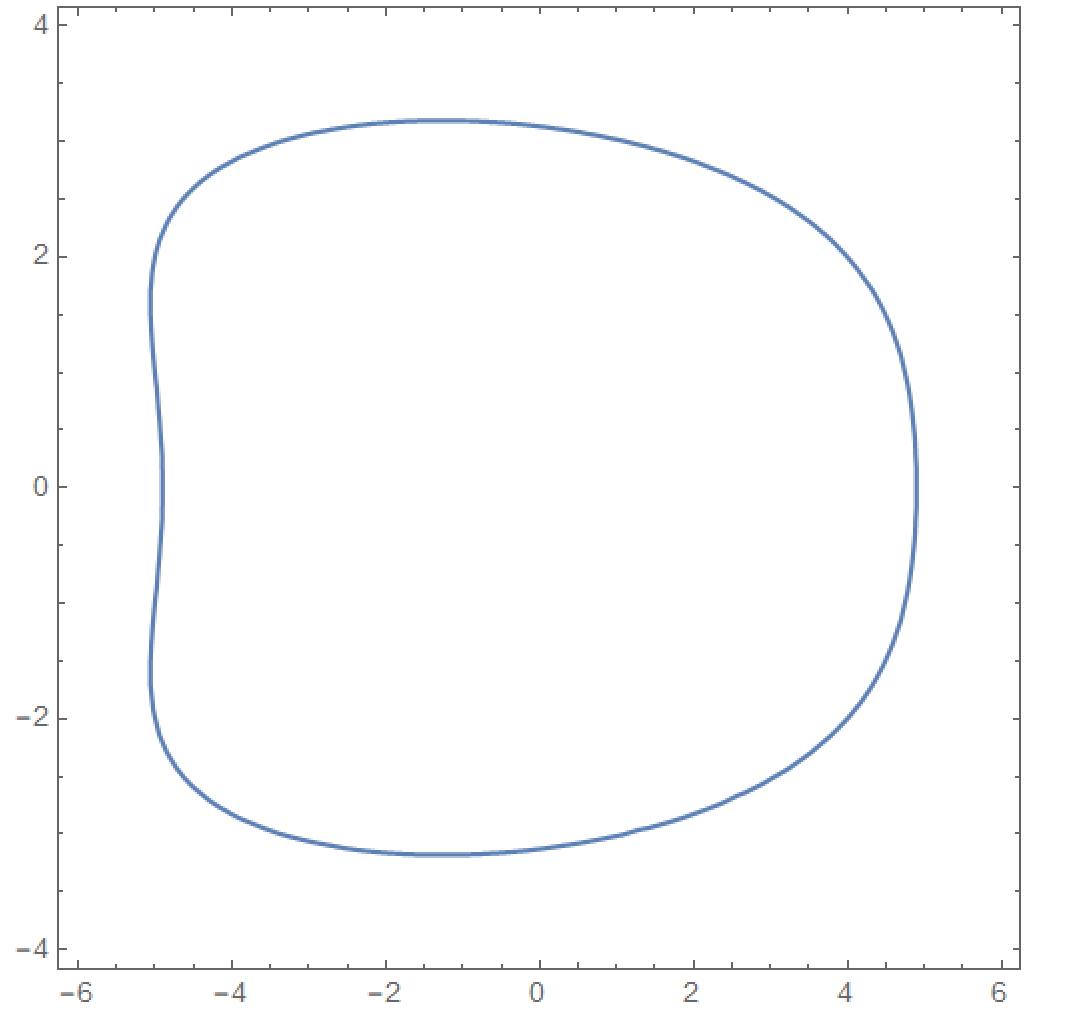
\includegraphics[scale=0.25]{eta-1.PNG}
    \raisebox{1.5cm}{\noindent\Huge=}
    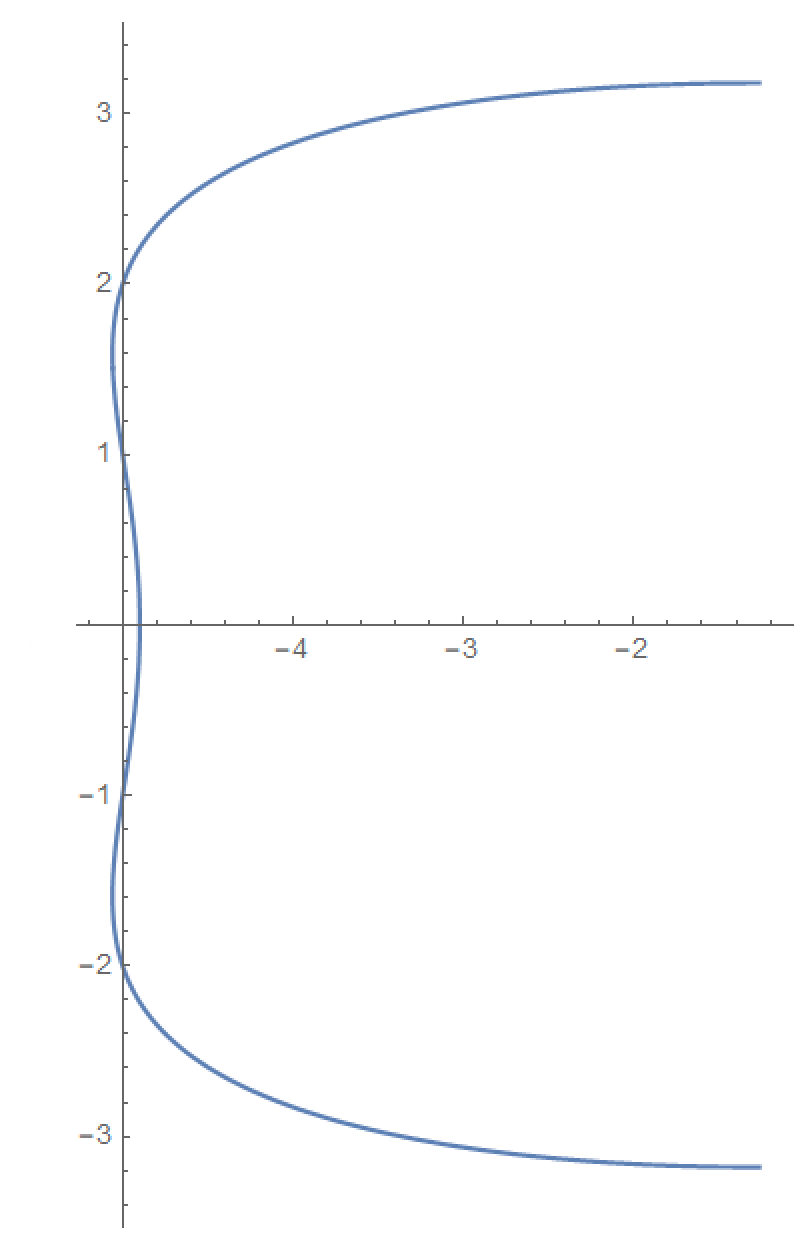
\includegraphics[scale=0.22]{eta-2.PNG}
    \raisebox{1.5cm}{\noindent\Huge$\cup$}
    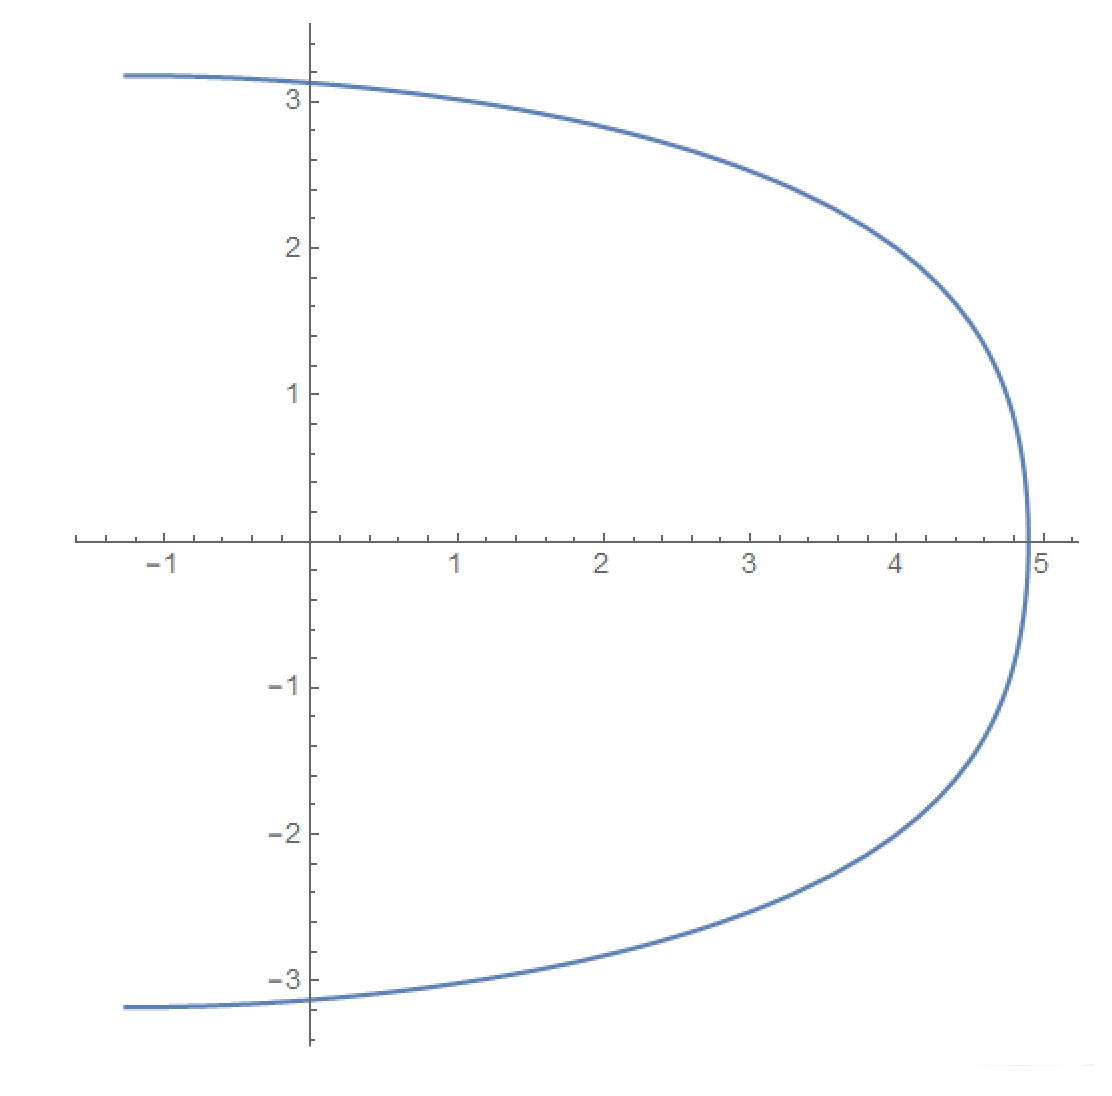
\includegraphics[scale=0.25]{eta-3.PNG}
\end{figure}

We ask what the Fourier transform of the volume element (or in this case the ``line element'') looks like. To find what $\Omega$ is we must find the ``charts'' with which we cover $\mathbb{S}$ (if we can always finitely cover $\mathbb{S}$ - which I believe we can - then $\mathbb{S}$ is compact... in which case what does that tell us?) \\

In any case, here's the parameterization I find for the zero set of $P(\eta) = 1$:
\begin{align*}
    \mathbb{S} = \lag \cup \mathcal{R}
\end{align*}
where $\lag$ denotes the left piece and $\mathcal{R}$ denotes the right piece:
\begin{align*}
    \lag &= \lc 
    \varphi_\lag(r) = \begin{pmatrix}
    \f{1}{8}\lb - r^2 - \sqrt{1536 - 15r^4} \rb \\ r
    \end{pmatrix}: r\in \lb -\sqrt[4]{512/5}, \sqrt[4]{512/5} \rb
    \rc\\
    \mathcal{R} &= \lc 
    \varphi_\mathcal{R}(r) = \begin{pmatrix}
    \f{1}{8}\lb - r^2 + \sqrt{1536 - 15r^4} \rb \\ r
    \end{pmatrix}: r\in \lb -\sqrt[4]{512/5}, \sqrt[4]{512/5} \rb
    \rc
\end{align*}
So, 
\begin{align*}
    J_{\vec{x}}(t) &= \int_{\lag} e^{-i \vec{x}\cdot t^E \vec{\eta}}\, d\Omega_{d-1}(\vec{\eta}) + \int_{\mathcal{R}} e^{-i \vec{x}\cdot t^E \vec{\eta}}\, d\Omega_{d-1}(\vec{\eta}) \\
    &= \int_{\lag} e^{-i \vec{x} \cdot t^E \varphi_{\lag}(r)}\, \det\lb E\varphi_{\lag}(r) \,\,\, \mathfrak{D}_r \varphi_{\lag}(r) \rb\, dr + \int_{\mathcal{R}} e^{-i \vec{x}\cdot t^E \varphi_{\mathcal{R}}(r)}\,  \det\lb E\varphi_{\mathcal{R}}(r) \,\,\, \mathfrak{D}_r \varphi(r) \rb\, dr.
\end{align*}

Calculate the determinant:
\begin{align*}
    \det\begin{bmatrix}
        E\varphi_{\lag/\mathcal{R}}(r) & \mathfrak{D}_r \varphi_{\lag/\mathcal{R}}(r)
    \end{bmatrix} 
    &=
    \det\begin{bmatrix}
    \f{1}{2}\f{1}{8}\lb - r^2 \mp \sqrt{1536 - 15r^4} \rb & \f{1}{4}r\lp -1 \pm \f{5\sqrt{3} r^2}{\sqrt{512 - 5r^4}} \rp \\
    \f{1}{4}r & 1
    \end{bmatrix}\\
    &= \f{\pm32\sqrt{3}}{\sqrt{512 - 5r^4}}\\
    \implies \abs{\det\lb E\varphi(r)\,\, \mathfrak{D}_r\varphi(r) \rb} &= \boxed{\f{32\sqrt{3}}{\sqrt{512 - 5r^4}}}
\end{align*}
Okay, back to the integral,
\begin{align*}
    J_{\vec{x}} (t) = \int_{r_\lag} e^{-i \vec{x} \cdot t^E \varphi_\lag(r)}\f{32\sqrt{3}}{\sqrt{512 - 5r^4}}\,dr + \int_{r_\mathcal{R}} e^{-i \vec{x} \cdot t^E \varphi_\mathcal{R}(r)}\f{32\sqrt{3}}{\sqrt{512 - 5r^4}}\,dr.
\end{align*}
Obviously there's more to unpack:
\begin{align*}
    \vec{x} \cdot t^E \varphi_\lag(r) =  x_1 t^{1/2}\f{1}{8}\lb -r^2 - \sqrt{1536 - 15r^4} \rb + x_2 t^{1/4} r
\end{align*}
Put this back into the integrals we get
\begin{align*}
    \int_\lag = \int_{-\sqrt[4]{512/5}}^{\sqrt[4]{512/5}} \f{32\sqrt{3}}{\sqrt{512 - 5r^4}} \exp \lb -i\lp x_1 t^{1/2}\f{1}{8}\lb -r^2 - \sqrt{1536 - 15r^4} \rb + x_2 t^{1/4} r \rp \rb\,dr\\
    \int_\mathcal{R} = \int_{-\sqrt[4]{512/5}}^{\sqrt[4]{512/5}}\f{32\sqrt{3}}{\sqrt{512 - 5r^4}} \exp \lb -i\lp x_1 t^{1/2}\f{1}{8}\lb -r^2 + \sqrt{1536 - 15r^4} \rb + x_2 t^{1/4} r \rp \rb\,dr
\end{align*}
and
\begin{align*}
    J_{\vec{x}}(t) = \int_{\lag\cup \mathcal{R}}\dots \implies H(\vec{x}) = \int^\infty_0 \,dt\, t^{\Tr E - 1}e^{-it}J_{\vec{x}}(t).
\end{align*}

Looking at $J_{\vec{x}} (t)$ now, can we have some kind of estimate on $\abs{J_{\vec{x}} (t)}$ as $t \to \infty$? I think we can, even though $J_{\vec{x}}(t)$ does not exactly have the same form as $I(\lambda)$. We can identify the function $\psi(x)$ with  $\f{32\sqrt{3}}{\sqrt{512 - 5r^4}}$, and have the phase $\Phi_\lambda(x)$ be identified with \begin{align*}
    \Phi_t(r) = x_1 t^{1/2}\f{1}{8}\lb -r^2 + \sqrt{1536 - 15r^4} \rb + x_2 t^{1/4}r.
\end{align*}
The terms $x_1,x_2$ comes from $H(\vec{x})$, but we hope that the estimate obtained will be independent of $\vec{x}$. I think a potential problem here is that $\psi(r)$ is not exactly ``slowly varying'' because $\psi'(r)$ blows up as $r$ approaches the limit points of  $(-\sqrt[4]{512/5},\sqrt[4]{512/5})$.\\

Anyway, the question now is we can use Stein's approach (or Vitturi's of integration by parts) to obtain an estimate/upper bound for the modulus of the integral 
\begin{align*}
\int_{r_\lag} \psi(r)e^{-i \Phi_{\vec{x},t}(r)}\,dr = \int_{-\sqrt[4]{512/5}}^{\sqrt[4]{512/5}} \f{32\sqrt{3}}{\sqrt{512 - 5r^4}} \exp \lb -i\lp x_1 t^{1/2}\f{1}{8}\lb -r^2 - \sqrt{1536 - 15r^4} \rb + x_2 t^{1/4} r \rp \rb\,dr
\end{align*}

To use Stein's theory/Vitturi's approach, we will want $\psi(r)$ to have compact support. In other words we want $\psi(-\sqrt[4]{512/5}) = \psi(\sqrt[4]{512/5}) = 0$. This is a problem because $\psi(r)$ blows up when $r$ approaches these values. \\



I can think of another way of writing the integral $\int_{\lag \cup \mathcal{R}}$ that involves the $\cos$, but I don't think if that's a good direction to head down because the final integral has $\psi(r) \sim \cos[f(r)]/f(r)$ where $f(r) = 0$ on the boundaries. \\





\hrule



\newpage

\texttt{April 17, 2020}:\\
$\,$\\

























So, we're trying to estimate:
\begin{equation*}
I=\left|\int_a^bt^{\alpha\Tr{E}-1}e^{it^\alpha}\,dt\right|
\end{equation*}
If I did things right, I obtain (just using the $f'$ part),
\begin{equation*}
I\leq \frac{4}{\alpha}\frac{b^{(\alpha\Tr{E}-1)}}{\inf_{t\in[a,b]}t^{(\alpha-1)}}
\end{equation*}
\begin{enumerate}
\item CASE 1: If $0<\alpha\leq \frac{1}{\Tr{E}}$ and $\Tr{E}\geq 1$ (which has generally been bad), then necessarily $0<\alpha<1$ and so
\begin{equation*}
\inf_{t\in[a,b]}t^{(\alpha-1)}=b^{(\alpha-1)}.
\end{equation*}
In this case, 
\begin{equation*}
I\leq \frac{4}{\alpha}b^{\alpha\Tr{E}-1}b^{(1-\alpha)}=\frac{4}{\alpha}b^{\alpha(\Tr{E}-1)}.
\end{equation*}
\item CASE 2: If $\Tr{E}<1$, choose $1<\alpha<\frac{1}{\Tr{E}}$. So,
\begin{equation*}
\inf_{t\in[a,b]}t^{\alpha-1}=a^{\alpha-1}. 
\end{equation*}
So,
\begin{equation*}
I\leq\frac{4}{\alpha}\frac{b^{(\alpha\Tr{E}-1)}}{a^{\alpha-1}}=\frac{4}{\alpha} a^{1-\alpha}b^{\alpha\Tr{E}-1}\leq \frac{4}{\alpha}a^{\alpha(\Tr E-1)}
\end{equation*}

\end{enumerate}




\hrule
$\,$\\
\noindnet \texttt{April 21, 2020:} \\


\noindent Here I'm trying to obtain an operator $L$ that works for the integral
\begin{align*}
    J_{\vec{x}}(t) = \int_{\mathbb{S}^{d-1}} e^{-i \vec{x} \cdot t^E \vec{\eta}}\,d\Omega_{d-1}(\eta).
\end{align*}
To make things match with what Stein has, I'm going to rewrite the integral above as 
\begin{align*}
    J_{\vec{x}}(t) = \int_{\mathbb{R}^{d-1}}\, d{\eta}\, \psi({\eta})\chi_{\mathbb{S}^{d-1}}({\eta})e^{-i {x}\cdot t^E {\eta}}  
\end{align*}
where $d\Omega_{d-1}(\eta) = \psi(\eta)\,d\eta$ and $\chi_{\mathbb{S}}(\eta)$ is the characteristic function for the set $\mathbb{S}$. To make things works as Stein described, we will want  $\chi_\mathbb{S}(\eta) \psi(\eta)$ to be smooth and compactly supported. We can mollify $\chi_\mathbb{S}$, but I don't know if $\psi(\eta)$ can be ``cured'' since as we have seen in the $\lag \cup \mathcal{R}$ example $\psi(\eta)$ can be pretty bad. \\

Anyway, I'll just go ahead and try. In Stein's descriptions, the oscillatory part of the integral looks like 
\begin{align*}
    e^{-i \lambda \Phi(x)}
\end{align*}
corresponding to which Stein introduces the operator 
\begin{align*}
    L = \f{1}{i\lambda}\f{\grad \Phi}{\abs{\grad \Phi}^2} \cdot \grad
\end{align*}
which has the property:
\begin{align*}
    L\lp e^{i \lambda \Phi(x)} \rp = e^{i \lambda \Phi(x)} \implies L^N\lp e^{i \lambda \Phi(x)} \rp = e^{i \lambda \Phi(x)}.
\end{align*}
With this, it is possible to transpose $L$ and let it act on the other piece of the integrand, each time bringing down a factor of $\lambda$. \\

We want to do the same thing here, except that we have a list of parameters instead of just a single number $\lambda$. In particular, our argument is $\eta$ and the parameters are $x$ and $t$. 

\begin{framed}
\noindent \textbf{Question:} Should we consider $\vec{x}$ or $t$ as the relevant parameter here? 
\end{framed}

Let's first consider $\vec{x}$ as the parameters. We know that for any $J_{\vec{x}}(t)$, the parameters $\vec{x}$ and $t$ are fixed. So, \textbf{assuming $t^E$ is diagonal}, we can take ``weighted'' gradients of the exponential piece with respect to the $x_i$'s or the $(t^E)_{ii}$ -- (diagonal) matrix elements of $t^E$. With respect to $x_i$ we can define
\begin{align*}
    \boxed{L_x \equiv \f{i}{\Tr (t^{2E})} \grad_x \lp x \cdot t^E \eta \rp \cdot \grad_x}
\end{align*}
where 
\begin{align*}
    \grad_x \equiv \sum^d_{i=1}\f{\hat\eta_i}{x_i}\p_{\eta_i}.
\end{align*}
Letting this act on $e^{-i x t^E \eta}$ we have
\begin{align*}
    L_x \lp e^{-i x\cdot  t^E \eta} \rp &= \f{i}{\Tr(t^{2E})}\lc \lb \sum^d_{i=1}\f{\hat\eta_i }{x_i}\p_{\eta_i}  \rb\lp x \cdot t^E \eta \rp \rc \cdot \lc  \lb \sum^d_{i=1}\f{\hat\eta_i }{x_i}\p_{\eta_i}  \rb e^{-i x \cdot t^E \eta} \rc\\
    &= \f{i(-i)}{\Tr(t^{2E})}\lc \lb \sum^d_{i=1}\f{\hat\eta_i }{x_i}\p_{\eta_i}  \rb\lp x \cdot t^E \eta \rp \rc \cdot \lc \lb \sum^d_{i=1}\f{\hat\eta_i }{x_i}\p_{\eta_i}  \rb\lp x \cdot t^E \eta \rp \rc e^{-i x \cdot t^E \eta}\\
    &= \f{1}{\Tr(t^{2E})} \lc \sum^d_{i=1} t^{E_{ii}} \hat\eta_i \rc \cdot \lc \sum^d_{i=1} t^{E_{ii}} \hat\eta_i \rc e^{-i x \cdot t^E \eta}\\
    &= \f{\Tr (t^{2E})}{ \Tr (t^{2E})} e^{-i x \cdot t^E \eta} \\
    &= e^{-i x \cdot t^E \eta}.
\end{align*}
Okay, so from here we have a similar thing as Stein did, which is that for any natural number $N$,
\begin{align*}
    L_x^N \lp  e^{-i x^E\eta} \rp &= e^{-i x^E\eta}
\end{align*}


\begin{framed}
\noindent \textbf{Question:} What is the transpose of $L_x$?
\end{framed}

\begin{framed}
\noindent \textbf{Question:} Will there be potential issues when we let $L_x$ act on the rest of the integrand? In particular, $L_x$ will introduce $1/x_i$ factors at various places. Will this a problem?
\end{framed}


Let's consider $t$ as the parameter. Then, we introduce the operator
\begin{align*}
    \boxed{L_t \equiv \f{i}{\norm{x}^2}\grad_t \lp x \cdot t^E \eta \rp  \cdot \grad_t}
\end{align*}
where (since $E$ is assumed to be diagonal)
\begin{align*}
    \grad_t \equiv \sum^d_{i=1} \f{\hat\eta_i}{t^{E_{ii}}} \p_{\eta_i} .
\end{align*}
Letting this act on $e^{-i x \cdot t^E \eta}$ we have
\begin{align*}
    L_t \lp e^{-i x \cdot t^E \eta} \rp
    &= \f{i}{\norm{x}^2} \lc \lb \sum^d_{i=1} \f{\hat\eta_i}{t^{E_{ii}}} \p_{\eta_i} \rb \lp x\cdot t^E \eta \rp \rc \cdot \lc \lb \sum^d_{i=1} \f{\hat\eta_i}{t^{E_{ii}}} \p_{\eta_i} \rb  \lp e^{-i x\cdot t^E \eta} \rp \rc\\
    &=  \f{i(-i)}{\norm{x}^2} \lc \lb \sum^d_{i=1} \f{\hat\eta_i}{t^{E_{ii}}} \p_{\eta_i}  \rb \lp x\cdot t^E \eta \rp \rc \cdot \lc \lb \sum^d_{i=1} \f{\hat\eta_i}{t^{E_{ii}}} \p_{\eta_i} \rb \lp x\cdot t^E \eta \rp \rc e^{-i x\cdot t^E \eta}\\
    &= \f{i(-i)}{\norm{x}^2} \lp \sum^d_{i=1} x_i^2 \rp e^{-i x\cdot t^E \eta}\\
    &= \f{i(-i)}{\norm{x}^2} \norm{x}^2 e^{-i x\cdot t^E \eta}\\
    &= e^{-i x\cdot t^E \eta}.
\end{align*}


Okay, so from here we have a similar things as Stein did, which is that for any natural number $N$,
\begin{align*}
    L_t^N \lp e^{-i x\cdot t^E \eta} \rp = e^{-i x \cdot t^E \eta}.
\end{align*}



\begin{framed}
\noindent \textbf{Question:} What is the transpose of $L_t$?
\end{framed}

\begin{framed}
\noindent \textbf{Question:} Will there be potential issues when we let $L_t$ act on the rest of the integrand? In particular, $L_t$ will introduce $1/t^{E_ii}$ factors at various places. Will this a problem?
\end{framed}


$\implies $ To find the transpose of $L_x$ or $L_t$ I think we'll have to be able to integrate by parts and require boundary terms be zero. 

$\,$\\

\hrule

$\,$\\



\newpage




\underline{\texttt{May 4, 2020:}} Notes on Theorem 14 in this \href{https://core.ac.uk/download/pdf/82381721.pdf}{\underline{paper}} by Iosevich and Sawyer.\\


\noindent We are interested in Theorem 14 of Iosevich and Sawyer because it might be applicable to our setup. I will give the statement first, then add what we will most likely care about.\\


\begin{defn}[Mixed homogeneous polynomial.]
    Suppose $a_1,\dots,a_n$ are positive integers. A function $f: \mathbb{R}^n \to \mathbb{R}$ is \textit{mixed homogeneous of degree} $(a_1,\dots,a_n)$ if for al $t>0$ and all $(x_1,\dots,x_n) \in \mathbb{R}^n$ we have
    \begin{align*}
        f\lp t^{1/a_1}x_1,\dots,t^{1/a_n}x_n \rp = tf(x_1,\dots,x_n).
    \end{align*}
\end{defn}

So, our $P$ is of course mixed homogeneous.  



\begin{thm}[THEOREM 14 of Iosevich and Sawyer] 
    Let $\Phi$ be a smooth function with the following properties. Suppose that after perhaps applying a rotation $\Phi(x) = Q(x) + R(x)$, where $Q$ is mixed homogeneous of degree $(a_1,\dots,a_n)$ with $(1/a_1) + \dots + (1/a_n) \leq 1$, $Q(x) \neq 0$ for $x\neq 0$ and $R$ satisfies 
    \begin{align*}
        \lim_{s\to 0} \f{R(s^{1/a_1} x_1, \dots, s^{1/a_n} x_n)}{s} = 0.
    \end{align*}
    Let $\mu$ denote the number of distinct $a_j$'s. Suppose that 
    \begin{align*}
    \int \abs{\Phi(x)}^{-\rho} \psi(x)\,dx < \infty,
    \end{align*}
    where $0 < \rho < 1/(\mu+1)$ and $\rho \leq (1/a_1)+\dots + (1/a_n)$. Let 
    \begin{align*}
        F(\xi,\lambda) = \int e^{i(x\cdot \xi + \lambda \Phi(x))}\psi(x)\,dx.
    \end{align*}
    Then if $\psi$ has sufficiently small support,
    \begin{align*}
        F(\xi,\lambda) \leq C(1+ \abs{\xi} + \abs{\lambda})^{-\rho}.
    \end{align*}
\end{thm}


\noindent To put the theorem into context, we can identify $F(\xi,\lambda)$ in the theorem with our $H(\vec{x})$ by setting $\lambda = 1$ and identifying $\Phi(x)$ with $P(x)$. (I think putting $\lambda = -1$ is fine too, because the oscillatory just goes in the opposite direction and doesn't affect convergence/boundedness). Next, because our $P(x)$ is positive homogeneous and $\Phi(x) = Q(x) + R(x)$, where $Q(x)$ is the mixed homogeneous piece and $R(x)$ is ``the rest,'' we can just assume $R(x) \equiv 0$. Remark 5 of the Iosevich paper says that the hypothesis $Q(x) \neq $ for $x\neq 0$ can be dropped if we assume $R \equiv 0$. Next, because our $H(\vec{x})$ looks like
\begin{align*}
    H(\vec{x}) = \int e^{\pm i(x\cdot \xi + P(x))}\,dx,
\end{align*}
the function $\psi(x)$ is either the constantly 1 function or the characteristic function on some ball which we will take to be infinity. This is something we will worry about later. Lastly, we also identify
\begin{align*}
    (1/a_1) + \dots + (1/a_n) \mbox{ with } \Tr E.
\end{align*}


With these identifications, we are interested in the specific case of 
\begin{align*}
    F(\xi, 1) = \int e^{i(x\cdot \xi + Q(x))}\psi(x)\,dx. 
\end{align*}
To use the theorem we probably want to check that 
\begin{align*}
    \int \abs{\Phi(x)}^{-\rho} \psi(x)\,dx < \infty
\end{align*}
where $0 < \rho < 1/(\mu+1)$ and $\rho \leq \Tr E $. The motivation for the integrability assumption in the theorem is given in the paper. It goes something like this:\\

Consider the integral
\begin{align*}
    \int_B e^{i\lambda Q(x)}\,dx
\end{align*}
where $Q$ is homogeneous of degree $m \geq 2$ and without loss of generality assume $Q \geq 0$ (these assumptions are both reasonable for our problem). $B$ is of course the unit ball. In polar coordinates in the integral is
\begin{align*}
    \int^1_0 \int_{\mathbb{S}^{n-1}}e^{i\lambda r^m Q(\omega)}r^{n-1}d\omega dr = \int^1_0 \int_{\{ \lambda Q(\omega) \leq 1 \}} + \int^1_0 \int_{\{ \lambda Q(\omega) > 1 \}} = \mbox{I} + \mbox{II}.
\end{align*}
Basically, $\abs{\mbox{I}}$ and $\abs{\mbox{II}}$ are $\leq C\lambda^{-\rho}$ provided 
\begin{align*}
    \int_{\mathbb{S}^{n-1}} Q(\omega)^{-\rho}d\omega < \infty.
\end{align*}
The calculation/proof for homogeneous $Q$ is shown, and the authors claim that the calculations for mixed homogeneous $Q$ are similar. \\

\noindent \textbf{Question/Comment:} While I believe our $P(x)$ satisfies the integrability assumption, I couldn't follow the calculations provided in the paper. \\




\noindent \begin{proof}[PROOF OF THEOREM 14]
    Assume without loss of generality that $Q(\omega) \geq 0$. This is a reasonable assumption for us because our $P$ is actually positive homogeneous. Also assume that $\mu= n$ where $\mu$ is the number of distinct $a_j$'s, and $n$ is the dimension. The general case requires some modifications to the proof below.\\
    
    To prove Theorem 14 we use the weighted polar coordinate system given by
    \begin{align*}
        x_i = r^{a_1/a_i} \omega_i
    \end{align*}
    where $r$ is the radial coordinate and $\omega = (\omega_1,\dots,\omega_n)$ is the standard coordinates on $\mathbb{S}^{n-1}$. The Jacobian of this change of variables is \begin{align*}
        g(\omega)r^{(a_1/a_2) + \dots + (a_1/a_n)}
    \end{align*}
    where $1 \leq g(\omega) \leq C$ (\href{http://matwbn.icm.edu.pl/ksiazki/sm/sm27/sm2713.pdf}{\underline{FaRi}} have checked this). With this we write
    \begin{align*}
        F(\xi,\lambda) 
        &= \int \psi(x)\exp\lb i\lp x\dot \xi + \lambda \Phi(x) \rp \rb\,dx\\
        &= \int_{\mathbb{S}^{n-1}}\int^\infty_0 \psi(r)g(\omega)r^{a_1/a_2 +\dots+ a_1/a_n} \exp\lb i\lp \sum^n_{i=1}r^{a_1/a_i}\omega_i\xi_i  + \lambda r^{a_1}\Phi(\omega) \rp\rb \,dr\,d\omega\\
        &= 
        \int_{\mathbb{R}^+}\int_{\lc \omega \in \mathbb{S}^{n-1}: \lambda Q(\omega) \leq 1 \rc}\dots \,dr\,d\omega + 
        \int_{\mathbb{R}^+}\int_{\lc \omega \in \mathbb{S}^{n-1}: \lambda Q(\omega) > 1 \rc}\dots \,dr\,d\omega\\
        &= F_1(\xi,\lambda) + F_2(\xi,\lambda).
    \end{align*}

    Now look at $F_1$:
    \begin{align*}
        \abs{F_1(\xi,\lambda)} \leq C'\abs{\lc \omega: \lambda Q(\omega) \leq 1 \rc} \leq \lambda^{-\rho}\int_{\mathbb{S}^{n-1}}Q^{-\rho}(\omega)\,d\omega\leq C\lambda^{-\rho}
    \end{align*}
    by assumption. \textbf{\textcolor{red}{Note:}} this is similar to the calculation done in the motivation, which is also where I couldn't follow...\\
    
    Suppose that I believe the ``easy'' part that $\abs{F_1} \leq C\lambda^{-\rho}$, consider $F_2$ where $\lambda Q(\omega) > 1$. For our purposes I will just assume $\Phi = Q + R \equiv Q$, i.e., $R\equiv 0$, in which case
    \begin{align*}
        F(\xi,\lambda) = \int_{\mathbb{S}^{n-1}}\int^\infty_0 \psi(r)g(\omega)r^{a_1/a_2 +\dots+ a_1/a_n} \exp\lb i\lp \sum^n_{i=1}r^{a_1/a_i}\omega_i\xi_i  + \lambda r^{a_1}Q(\omega) \rp\rb \,dr\,d\omega
    \end{align*}
    where I just swapped out $\Phi$ for $Q$ and assumed that $\psi$ is radial. \textcolor{red}{\textbf{Note:}} I believe we can make this radial assumption because any function $\psi(x)$ can be approximated by radial function(?) \\
    
    Next, let $\psi_0 \in C^\infty_0(\mathbb{R})$ be a smooth cutoff function supported in the interval $[1/2,4]$ such that $\sum_k \psi_0(2^k s) \equiv 1$ (partition of unity) and let 
    \begin{align*}
        F_k(\xi,\lambda) = \int_{\mathbb{S}^{n-1}}\int^\infty_0 \psi_0(2^k r)g(\omega)r^{a_1/a_2 +\dots+ a_1/a_n} \exp\lb i\lp \sum^n_{i=1}r^{a_1/a_i}\omega_i\xi_i  + \lambda r^{a_1}Q(\omega) \rp\rb \,dr\,d\omega
    \end{align*}
    Define
    \begin{align*}
    G_k(r,\omega,\xi,\lambda) = \int^\infty_0 \psi_0(2^k r) r^{a_1/a_2 +\dots+ a_1/a_n} \exp\lb i\lp \sum^n_{i=1}r^{a_1/a_i}\omega_i\xi_i  + \lambda r^{a_1}Q(\omega) \rp\rb \,dr
    \end{align*}
    so that 
    \begin{align*}
        F_k(\xi,\lambda) = \int_{\mathbb{S}^{n-1}}G_k(r,\omega,\xi,\lambda) g(\omega)\,d\omega.
    \end{align*}
    Okay, consider another change of variables $r \to 2^{-k}r$ which results in a scaling factor of $2^{-k(1+a_1/a_2) + \dots + (a_1/a_n)}$, so that
    \begin{align*}
    G_k(r,\omega,\xi,\lambda) = &2^{-k(1+a_1/a_2) + \dots + (a_1/a_n)} \times \\&\int_0^\infty r^{(a_1/a_2)+\dots + (a_1/a_n)}\psi_0(r)\exp\lb i\lp \sum^n_{i=1}r^{a_1/a_i}2^{-k(a_1/a_{i})}\omega_i \xi_i  + 2^{-ka_1}r^{a_1}\lambda Q(\omega)\rp\rb \,dr
    \end{align*}
    We can identify this as Fourier transform of a smooth measure supported on the curve
    \begin{align*}
        \Gamma(r) = \lp r, r^{a_1/a_2}, \dots, r^{a_1/a_n},r^{a_1} \rp
    \end{align*}
    evaluated at
    \begin{align*}
        \lp 2^{-k}\omega_1\xi_1, \dots, 2^{-k(a_1/a_n)}\omega_n \xi_n, 2^{-ka_1}\lambda Q(\omega) \rp.
    \end{align*}
        
    
    
    
    
    
\end{proof}






\newpage







\texttt{June 12, 2020}









































\newpage

\section{Examples}
I was going to send you an email with this document and the new images attached, but it (as usual) got too long. So I decided to put everything into this document instead.  \\


\noindent \textbf{0.} The $\phi : \mathbb{Z}^2 \to \mathbb{C}$ that is used in this document is given by:
\begin{align}
\begin{cases}
\begin{alignedat}{2}
\f{301}{384} - \f{7i}{48}, &\quad (x,y) = (0,0)\\[10pt]
\f{7}{96} + \f{i}{24},& \quad (x,y) = (-1,0)\\[10pt]
\f{3}{32} + \f{i}{24},& \quad (x,y) = (1,0)\\[10pt]
-\f{1}{48}, &\quad (x,y) = (2,0)\\[10pt]
-\f{1}{48}, &\quad (x,y) = (-2,0)\\[10pt]
\f{7}{96} + \f{i}{24}, &\quad (x,y) = (0,1)\\[10pt]
\f{7}{96} + \f{i}{24}, &\quad (x,y) = (0,-1)\\[10pt]
-\f{7}{192} - \f{i}{96}, &\quad (x,y) = (0,2)\\[10pt]
-\f{7}{192} - \f{i}{96}, &\quad (x,y) = (0,-2)\\[10pt]
\f{1}{96}, &\quad (x,y) = (0,3)\\[10pt]
\f{1}{96}, &\quad (x,y) = (0,-3)\\[10pt]
-\f{1}{768}, &\quad (x,y) = (0,4)\\[10pt]
-\f{1}{768}, &\quad (x,y) = (0,-4)\\[10pt]
\f{1}{192}, &\quad (x,y) = (-1,-1)\\[10pt]
\f{1}{192}, &\quad (x,y) = (-1,1)\\[10pt]
-\f{1}{192}, &\quad (x,y) = (1,1)\\[10pt]
-\f{1}{192}, &\quad (x,y) = (1,-1)
\end{alignedat}
\end{cases}
\end{align}


\newpage



\noindent \textbf{1.}  


And so the FT of $\phi$, or $\hat\phi$, is the following: 
\begin{align}
\boxed{\hat{\phi}(\xi_1,\xi_2) =   \f{1}{3} \lp 3 - \f{i}{2}\sin^2(\xi_1/2) - \sin^4(\xi_1/2) - \f{i}{2}\sin^4(\xi_2/2) - \sin^8(\xi_2/2) - \f{i}{16}(\sin \xi_1 \cos \xi_2 - \sin \xi_1) \rp}
\end{align}

Taylor expanding this around $(0,0)$ gives 
\begin{align}
\left(1-\frac{i\xi_2^4}{96}+\frac{i\xi_2^6}{576}+ \mathcal{O}\left( \xi_2^7\right)\right) + \xi_1 \left(\frac{i  \xi_2^2}{96}-\frac{i  \xi_2^4}{1152}+\frac{i  \xi_2^6}{34560}+ \mathcal{O}\left( \xi_2^7 \right)\right)-\frac{i\xi_1^2}{24}\nn\\
+ \xi_1^3 \left(-\frac{i\xi_2^2}{576}+\frac{i\xi_2^4}{6912}-\frac{i\xi_2^6}{207360}+ \mathcal{O}\left( \xi_2^7\right)\right)-\left(\frac{1}{48}-\frac{i}{288}\right)  \xi_1^4+ \mathcal{O}\left( \xi_1^5\right).
\end{align}

I have checked that $\hat{\phi}(0,0) = 1$. With this, Taylor-expanding
\begin{align}
\log\lp \f{\hat\phi((\xi_1,\xi_2) + (0,0))}{\hat\phi(0,0)} \rp
\end{align} 
gives
\begin{align}
\left(-\frac{i  \xi_2^4}{96}+\mathcal{O}\left( \xi_2^5\right)\right)+ \xi_1 \left(\frac{i  \xi_2^2}{96}-\frac{i  \xi_2^4}{1152}+\mathcal{O}\left( \xi_2^5\right)\right)+ \xi_1^2 \left(-\frac{i}{24}+\frac{ \xi_2^4}{2048}+\mathcal{O}\left( \xi_2^5\right)\right)+\mathcal{O}\left( \xi_1^3\right).
\end{align}
With $\vec\xi \equiv (\xi_1,\xi_2)$, we read off $iP(\vec\xi)$:
\begin{align}
\boxed{\Pi(\vec{\xi}) = iP(\vec{\xi}) = -\frac{i  \xi_2^4}{96} + \frac{i \xi_1  \xi_2^2}{96} -\f{i\xi_1^2}{24} }
\end{align}

Once $\cos$ and $\sin$ in $\hat{\phi}$ have been replaced by $e^{i\dots}$ we can write $\hat\phi$ as
\begin{align}
&\frac{1}{192} e^{i \xi_2-i \xi_1} -\frac{1}{192} e^{i \xi_1+i \xi_2} +\frac{1}{192} e^{-i \xi_1-i \xi_2} -\frac{1}{192} e^{i \xi_1-i\xi_2}+\left(\frac{3}{32}+\frac{i}{24}\right) e^{i \xi_1}\nn\\
&+\left(\frac{7}{96}+\frac{i}{24}\right) e^{-i \xi_1}-\frac{1}{48} e^{-2 i \xi_1}-\frac{1}{48} e^{2 i \xi_1}+\left(\frac{7}{96}+\frac{i}{24}\right) e^{-i \xi_2}-\frac{1}{768} e^{-4 i \xi_2}+\frac{1}{96} e^{-3 i \xi_2}\nn\\
&-\left(\frac{7}{192}+\frac{i}{96}\right) e^{-2 i \xi_2}+\left(\frac{7}{96}+\frac{i}{24}\right) e^{i \xi_2}-\left(\frac{7}{192}+\frac{i}{96}\right) e^{2 i \xi_2}+\frac{1}{96} e^{3 i \xi_2}-\frac{1}{768} e^{4 i \xi_2}+\left(\frac{301}{384}-\frac{7 i}{48}\right)
\end{align}
from which we can read off the values of $\phi: \mathbb{Z}^2 \to \mathbb{C}$. 
















\newpage











\noindent \textbf{2.} I rescaled the $x,y$ in the previous $H(x,y)$ with $t = 100$ and got good correspondence after some hours of numerical integration. ($t$ here appears in $H^t_p$ and $t^E$ in the paper).  I wish I had thought about the possibility that the stretching could be so extreme that the peaks appear rotated earlier...\\

Here are the images. Purple-ly plots are convolution powers with $n = 100$. Green-ish plots are the approximated attractor $H^t_P(x,y)$ with $t = 100$. (I don't know what the exact correspondence between $t$ and $n$ is for now, but I think setting them equal is an o.k. starting point.)

\begin{figure}[!htb]
	\centering
	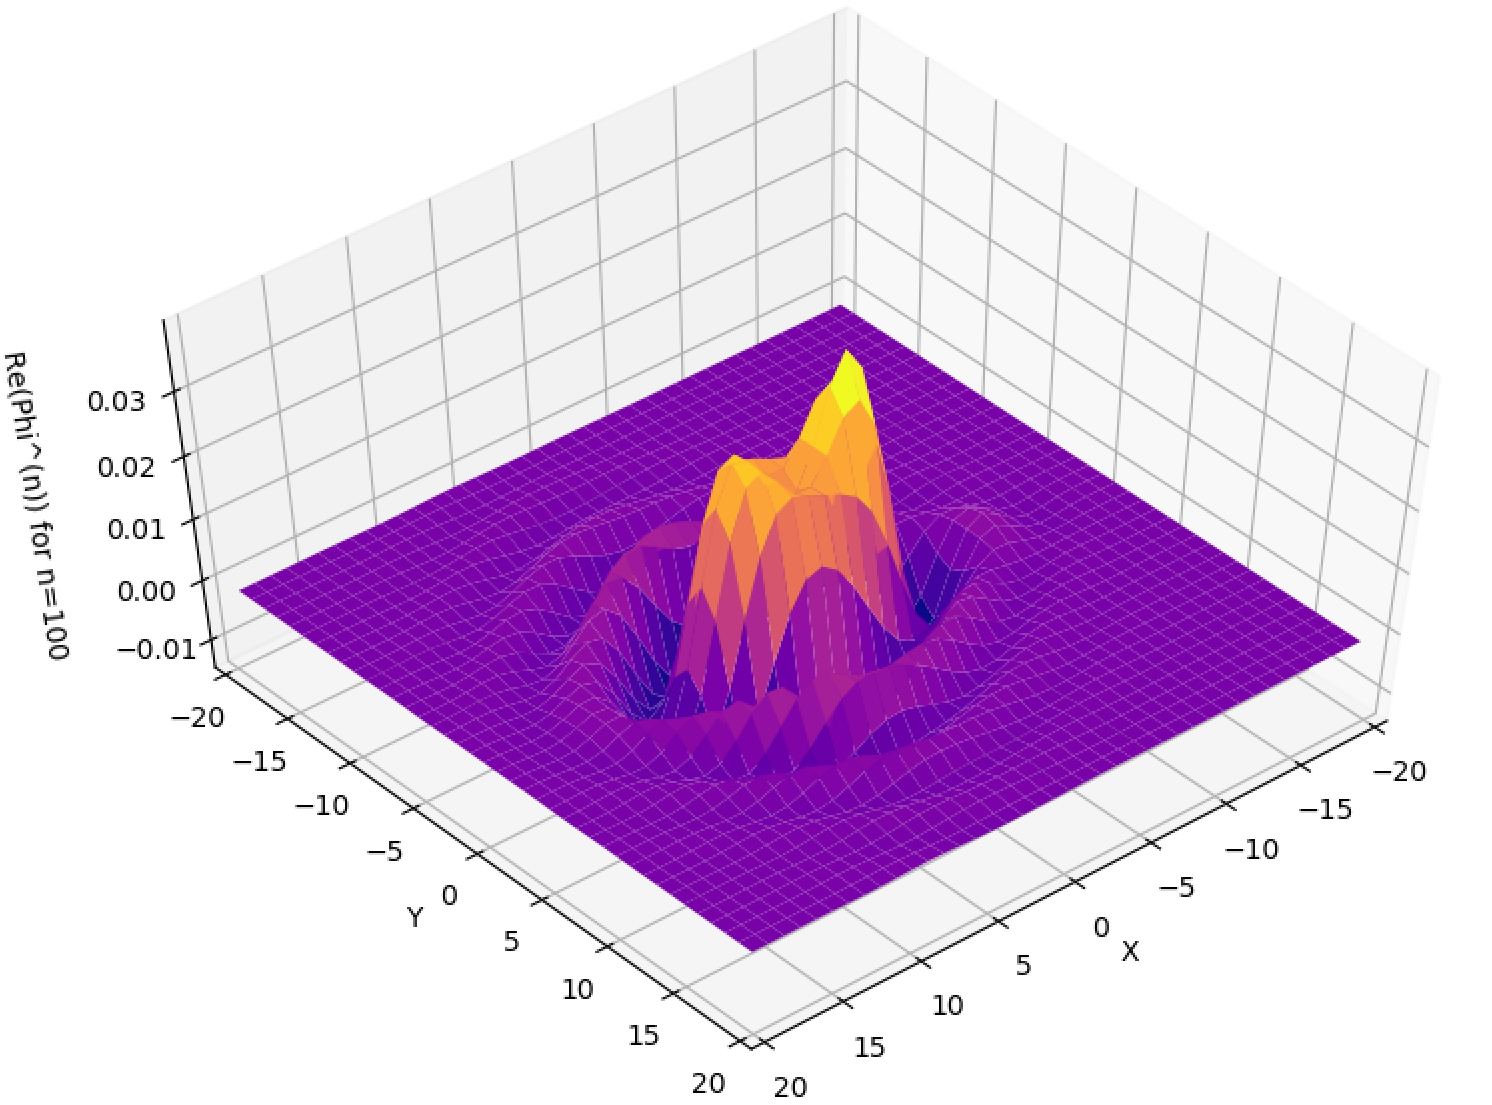
\includegraphics[scale=0.4]{conv}
	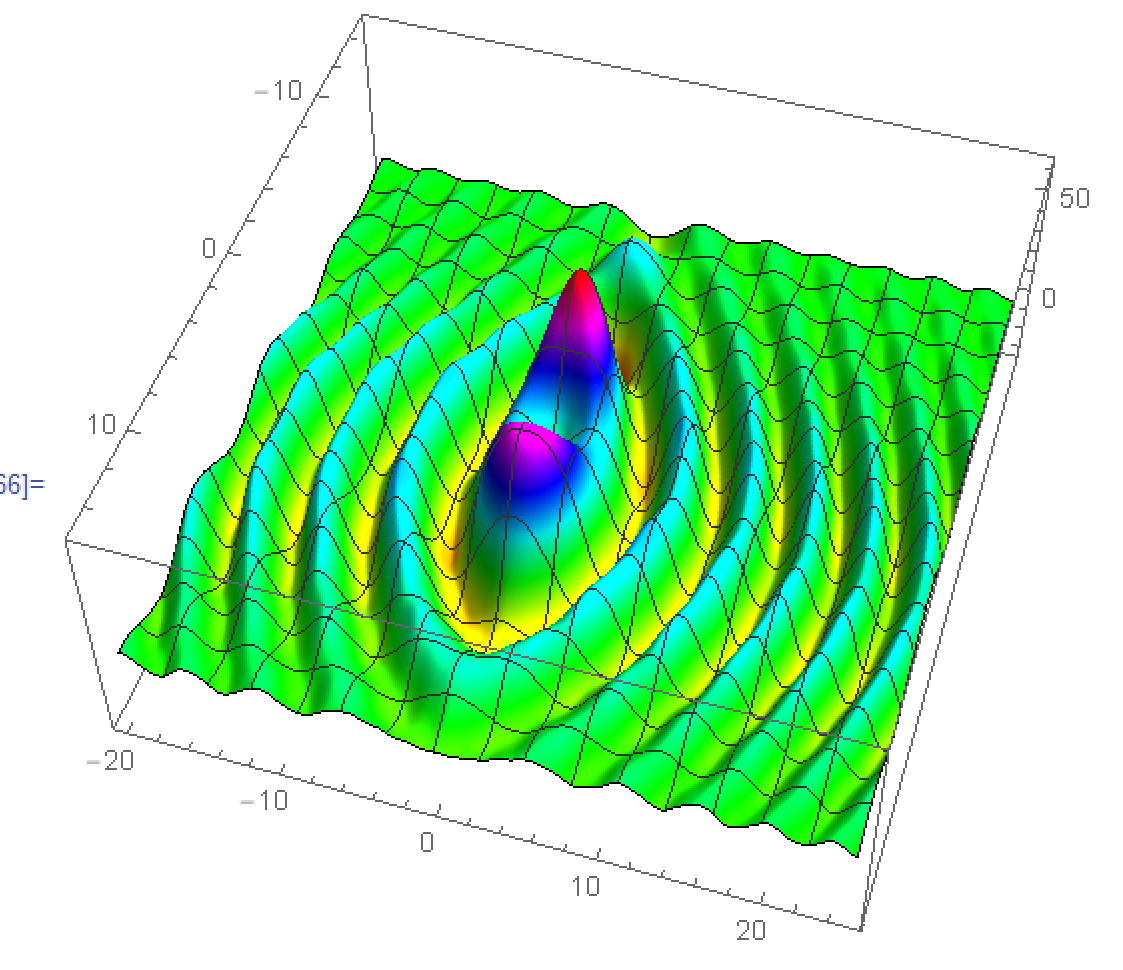
\includegraphics[scale=0.45]{conv-1}\\
	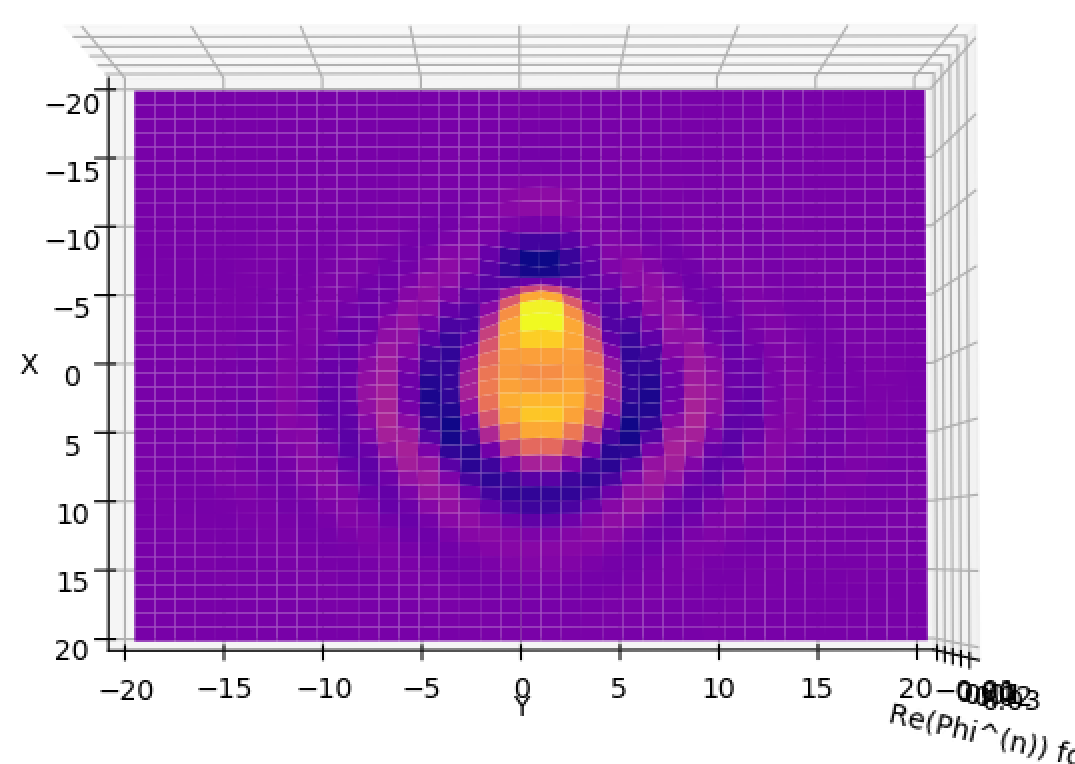
\includegraphics[scale=0.55]{conv-2}
	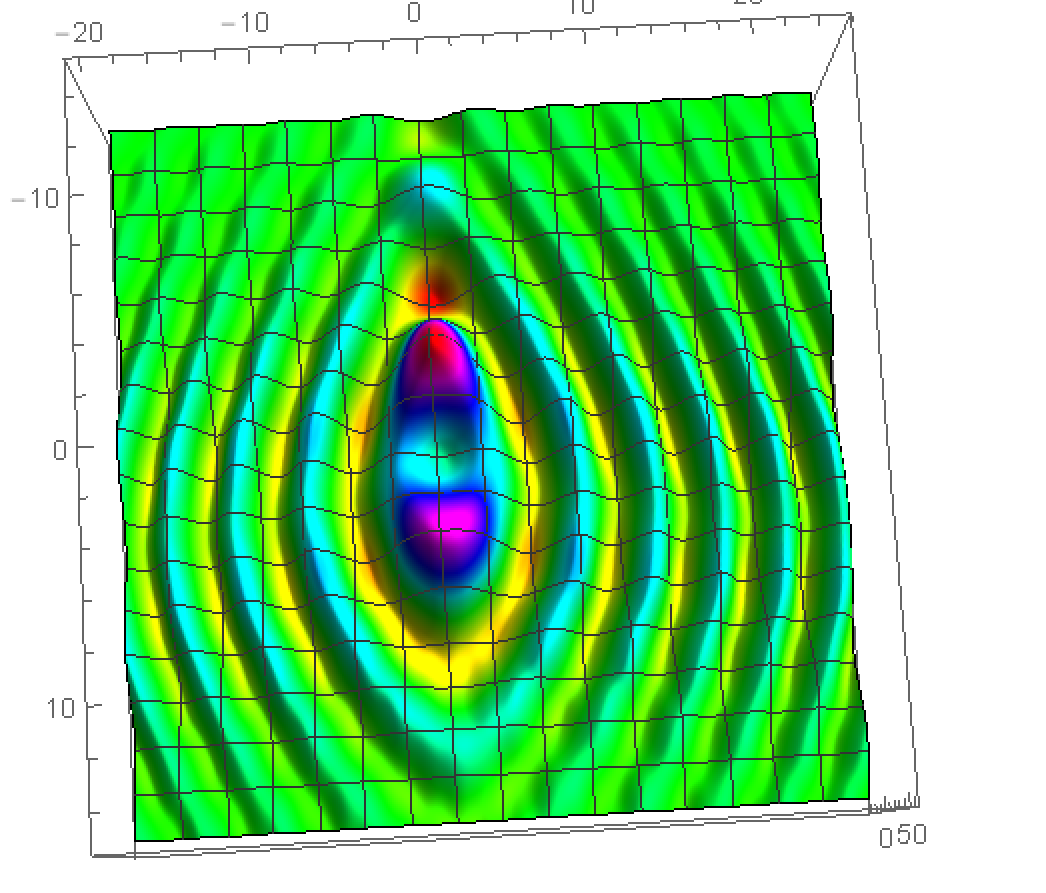
\includegraphics[scale=0.5]{conv-3}\\
	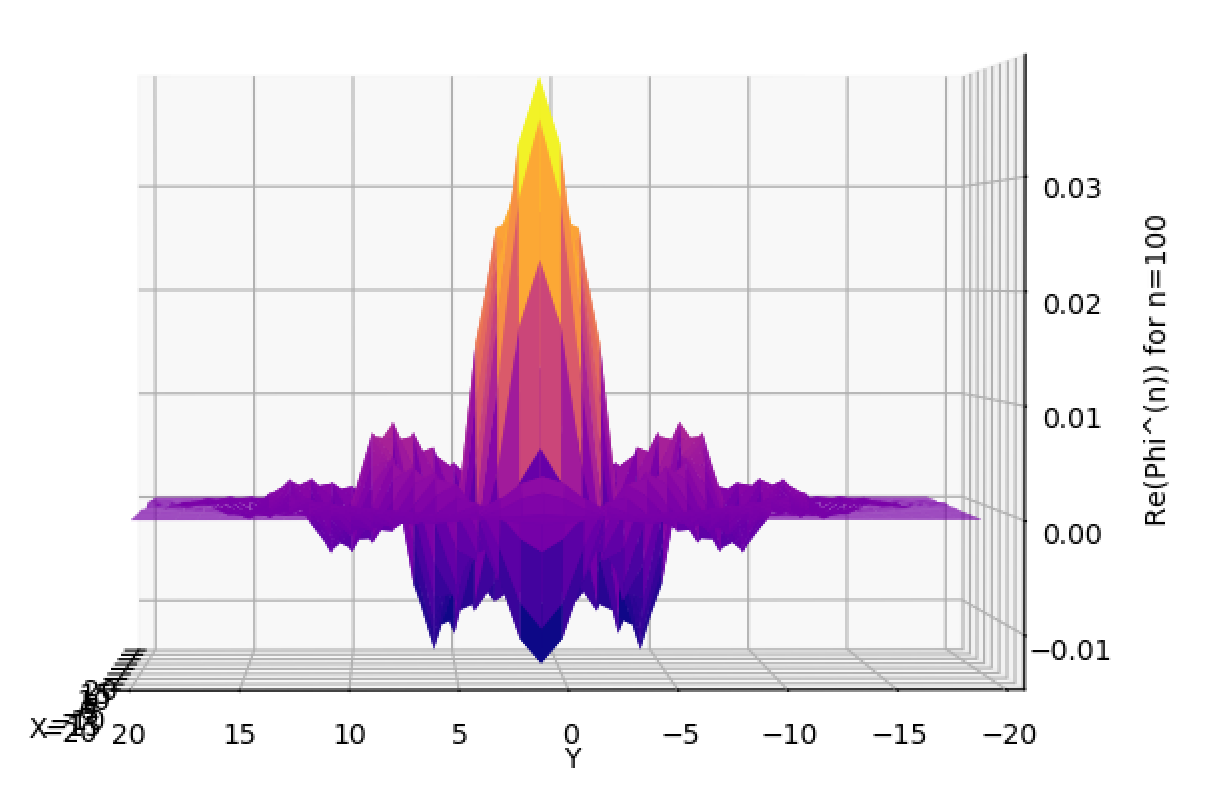
\includegraphics[scale=0.4]{conv-4}
	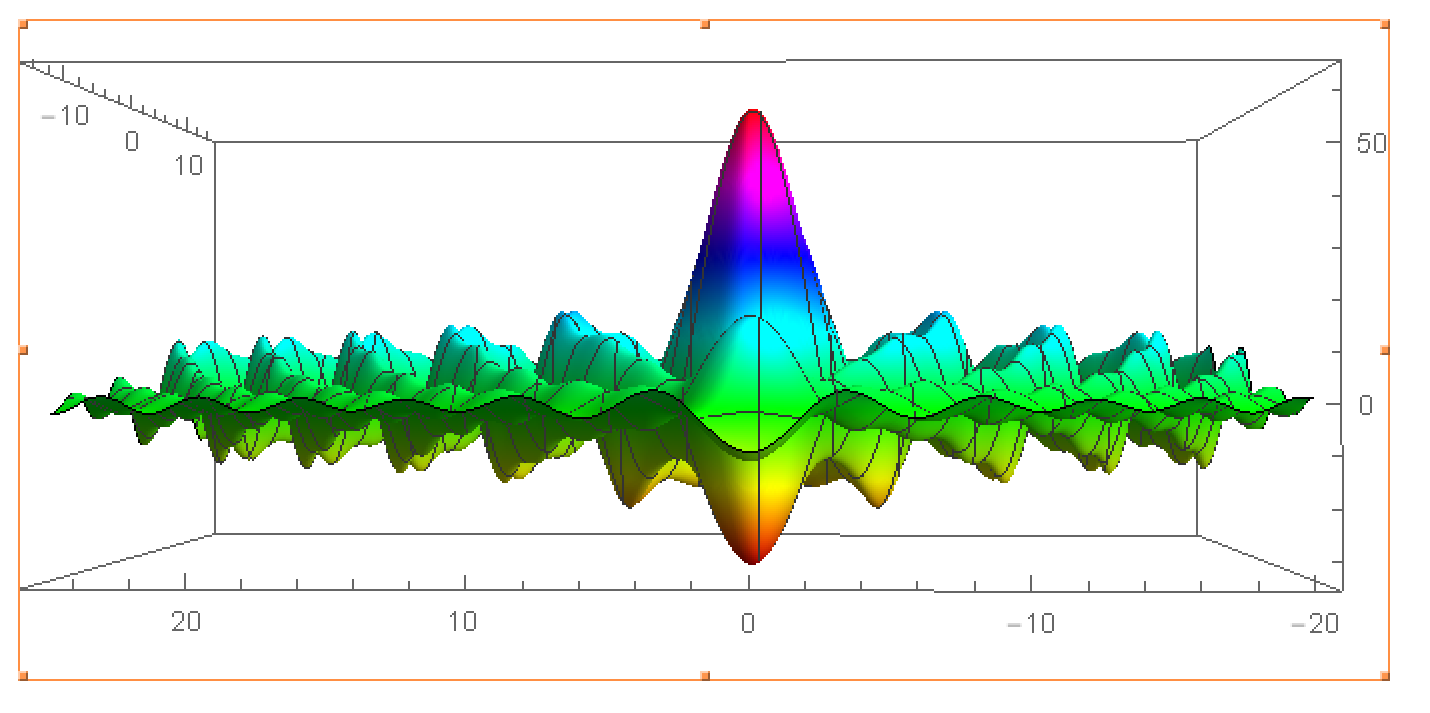
\includegraphics[scale=0.4]{conv-5}
\end{figure}








\newpage

\noindent \textbf{3.} I'm still running the calculations for $H^t_P(x,y)$ again with $t = 100$. The output looks good. I'm integrating in ``batches'' and will aggregate the data as I go along. This should give us a lot of data for future stretching/contracting/scaling at different values of $t$. Below is the first few batches (around the origin). The peaks have the correct orientation, and are very much like the convolution powers we've been generating!

\begin{figure}[!htb]
	\centering
	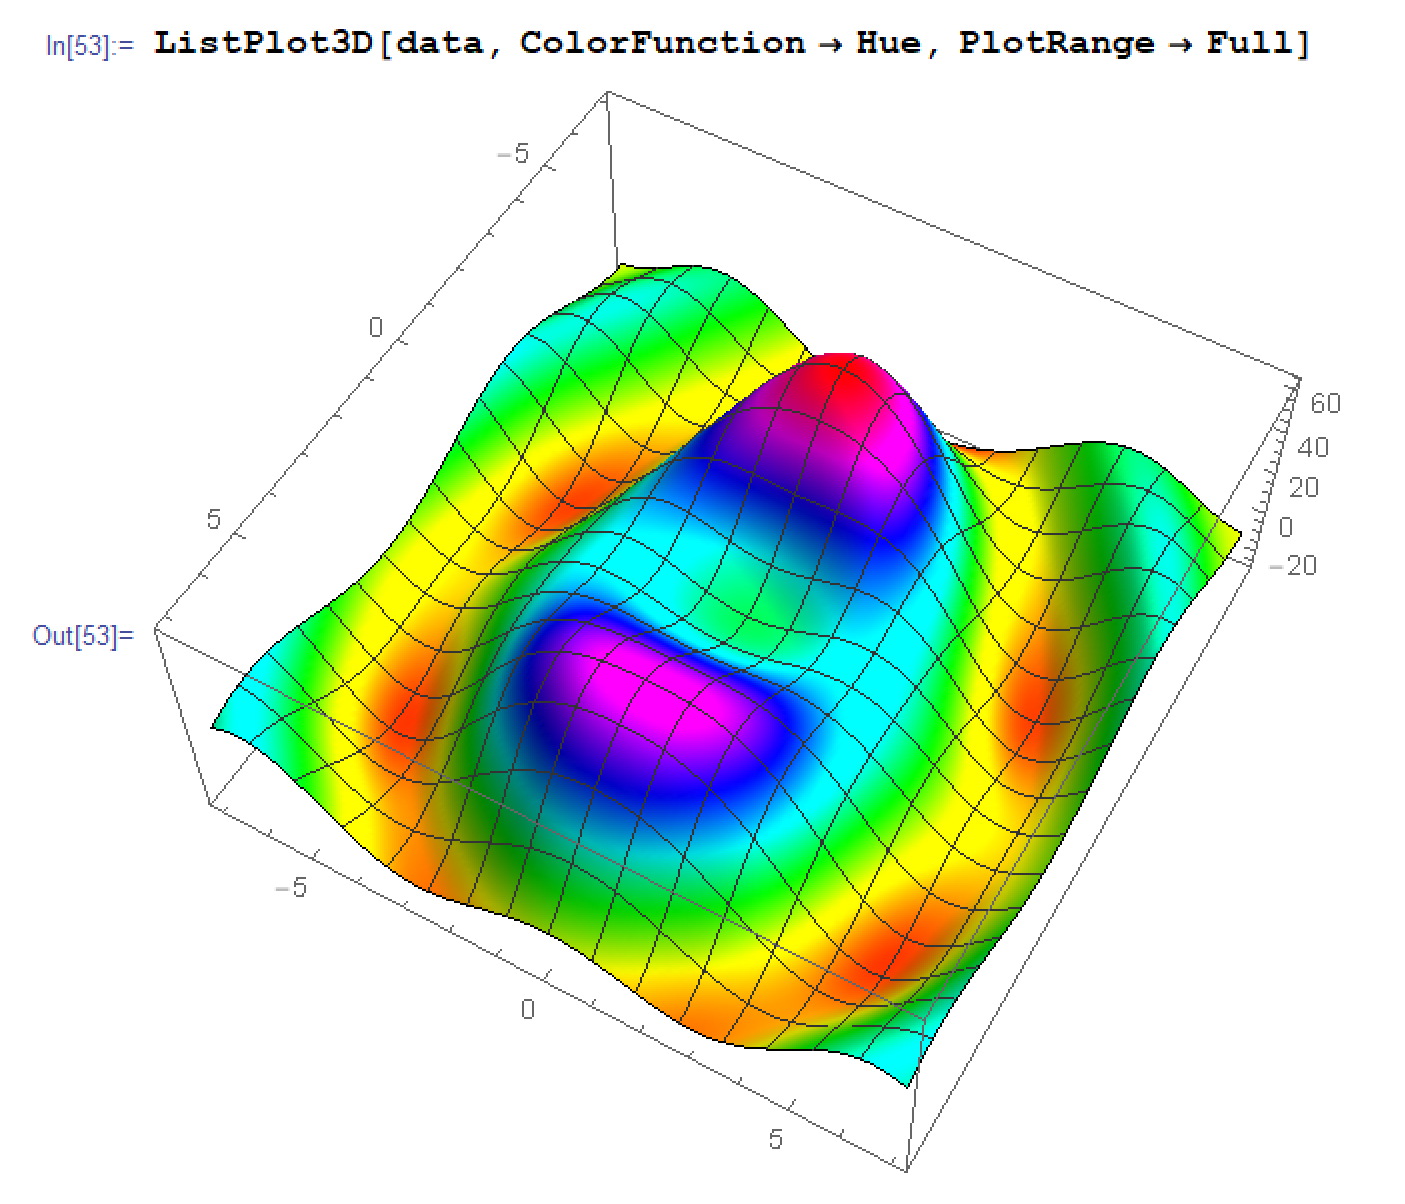
\includegraphics[scale=0.15]{conv-6}
	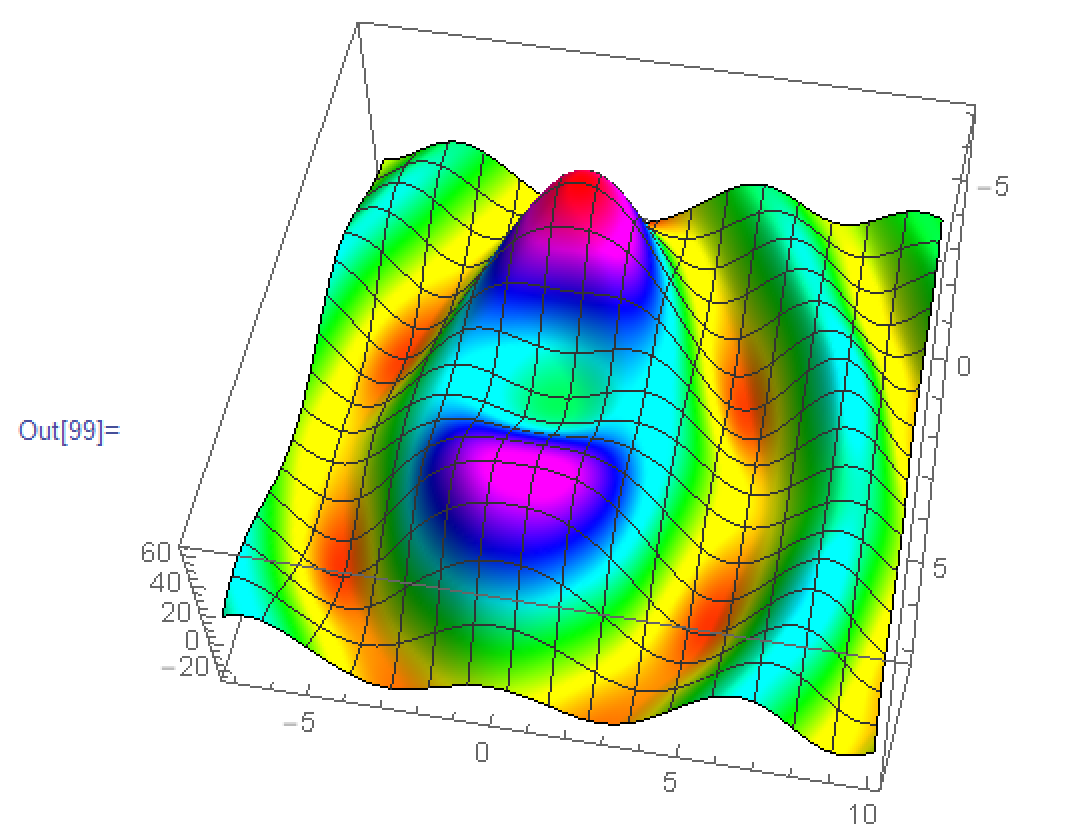
\includegraphics[scale=0.2]{conv-7}
	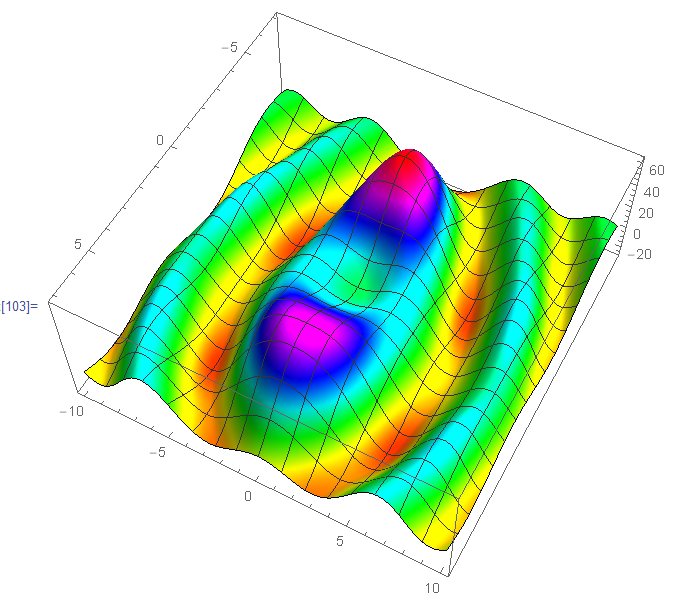
\includegraphics[scale=0.3]{conv-8}
\end{figure}


This is what I have as of March 9 and March 21, 2020:
\begin{figure}[!htb]
	\centering
	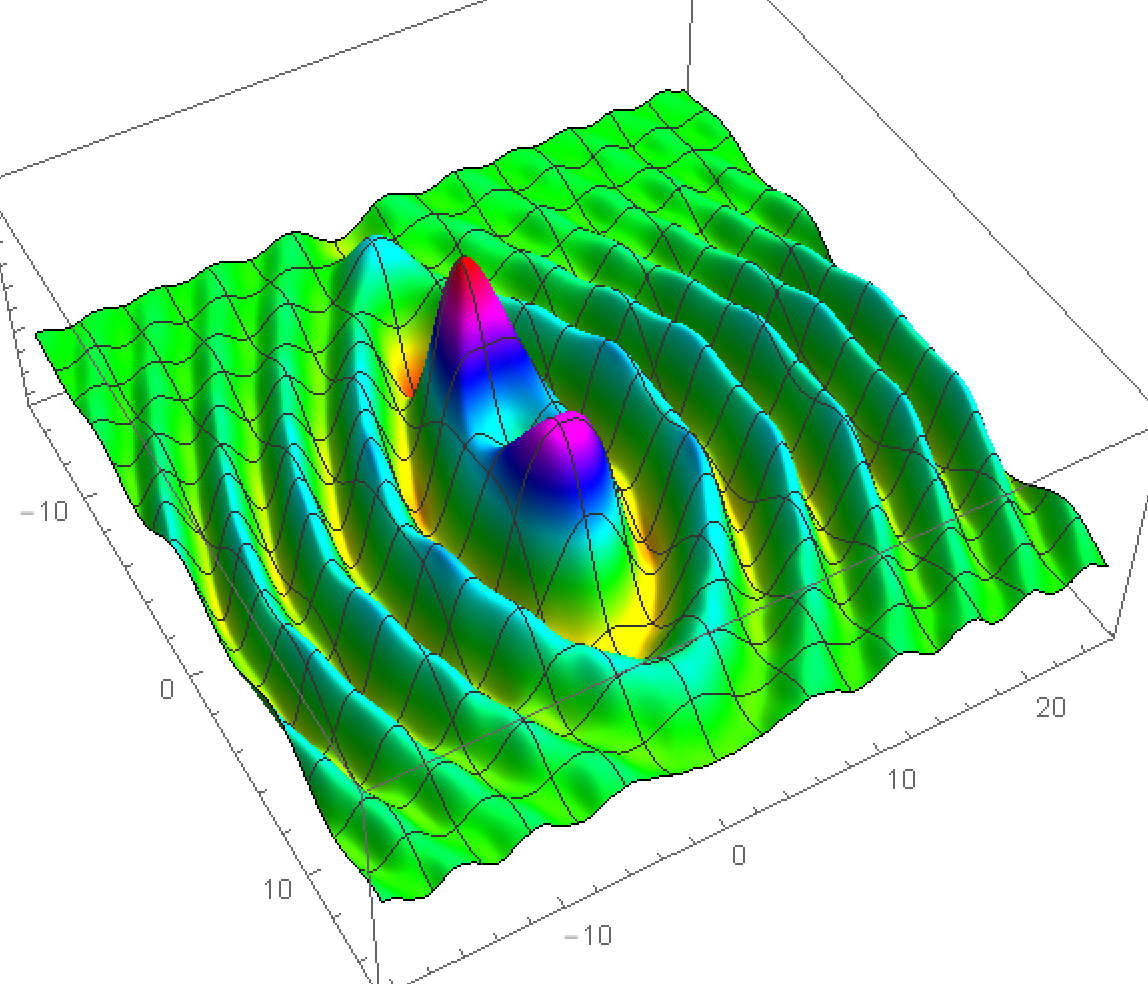
\includegraphics[scale=0.45]{conv-9}
	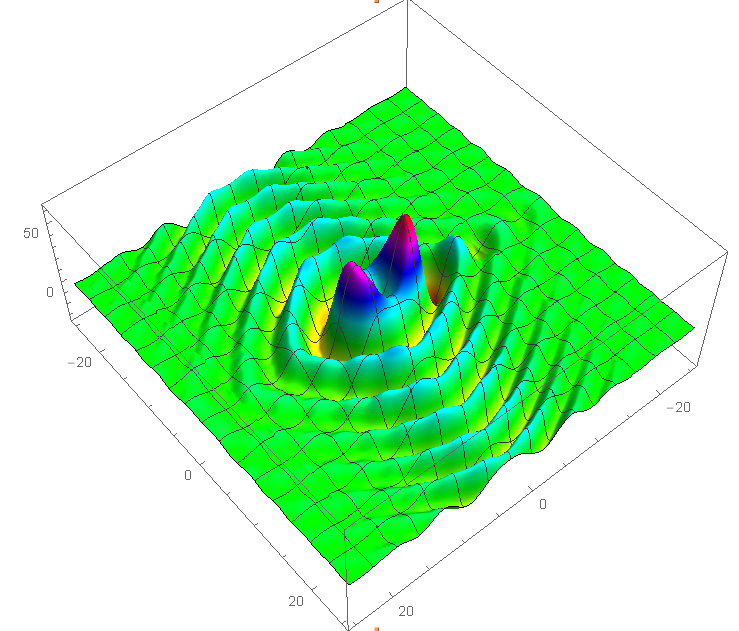
\includegraphics[scale=0.4]{conv-10}
\end{figure}



There are about $2\times 10^5$ data points in the second figure. 







\newpage

\noindent \textbf{4.} Here's the Python code I use to calculate the convolution powers
\begin{lstlisting}
import numpy as np
import matplotlib.pyplot as plt
from scipy import signal
from matplotlib import cm, colors
from mpl_toolkits.mplot3d.axes3d import Axes3D
import operator
import time
from numpy import unravel_index


def fast_convolve(n_times, support_bound, drift):
	Phi = np.zeros(shape=(9,9),dtype=np.complex_)

	Phi[ 0+9//2][ 0+9//2]  = complex(301/384,-7/48)
	Phi[ 0+9//2][-1+9//2]  = complex(7/96,1/24)     
	Phi[ 0+9//2][ 1+9//2]  = complex(3/32,1/24)      
	Phi[ 0+9//2][ 2+9//2]  = -1/48               
	Phi[ 0+9//2][-2+9//2]  = -1/48
	Phi[ 1+9//2][ 0+9//2]  = complex(7/96,1/24)
	Phi[-1+9//2][ 0+9//2]  = complex(7/96,1/24)
	Phi[ 2+9//2][ 0+9//2]  = -complex(7/192,1/96)
	Phi[-2+9//2][ 0+9//2]  = -complex(7/192,1/96)
	Phi[ 3+9//2][ 0+9//2]  = 1/96
	Phi[-3+9//2][ 0+9//2]  = 1/96
	Phi[ 4+9//2][ 0+9//2]  = -1/768
	Phi[-4+9//2][ 0+9//2]  = -1/768
	Phi[-1+9//2][-1+9//2]  =  1/192
	Phi[ 1+9//2][-1+9//2]  =  1/192
	Phi[ 1+9//2][ 1+9//2]  = -1/192
	Phi[-1+9//2][ 1+9//2]  = -1/192

	conv_power = np.copy(Phi)
	offset = np.array([0,0])

	i=0
	if drift:
		while i < n_times:
			i += 1
			init_vec = unravel_index(np.absolute(conv_power).argmax(), np.absolute(conv_power).shape)
			conv_power = signal.convolve2d(Phi, conv_power, 'full')
			after_vec = unravel_index(np.absolute(conv_power).argmax(), np.absolute(conv_power).shape)
			offset += np.subtract(init_vec , after_vec)

			dim_f = np.shape(conv_power)
	
			if dim_f[0] > support_bound or dim_f[0] > support_bound:
				conv_power = crop(conv_power, support_bound)
	else:
		while i < n_times:
			i += 1
			conv_power = signal.convolve2d(Phi, conv_power, 'full')
			dim_f = np.shape(conv_power)

			if dim_f[0] > support_bound or dim_f[0] > support_bound:
				conv_power = cropND(conv_power, support_bound)
return conv_power

def cropND(img, sup_bd):
	if sup_bd < np.shape(img)[0] and sup_bd < np.shape(img)[1]:
	dim = np.shape(img)
	return img[(dim[0]//2)-sup_bd//2:(dim[0]//2)+sup_bd//2,
		(dim[1]//2)-sup_bd//2:(dim[1]//2)+sup_bd//2]

def crop(img, sup_bd):
	center = unravel_index(np.absolute(img).argmax(), np.absolute(img).shape)
	return img[center[0]-sup_bd//2:center[0]+sup_bd//2,
		center[1]-sup_bd//2:center[1]+sup_bd//2]

if __name__ == '__main__':

while True:

	n_times = int(input('Convolve how many times? '))
	support_bound = int(input('NxN suppport bound, N = '))
	drift_ans = str(input('Expect asymetric drift? [y/n]: '))
	print('Calculating...')
	start = time.time()

	if drift_ans == 'y':
		drift = True
	elif drift_ans == 'n':
		drift = False
	else:
		print('WARNING: Write "y" for YES and "n" for NO.')
		print('------------------------------------------')
		print('\n')
		continue

	data = np.real(fast_convolve(n_times, support_bound, drift))
	dim = np.shape(data)
	x = range((-dim[0]//2)+1,(dim[0]//2)+1)
	y = range((-dim[1]//2)+1,(dim[1]//2)+1)

	hf = plt.figure()
	ha = hf.add_subplot(projection='3d')
	ha.set_xlim(-np.shape(data)[0]//2, np.shape(data)[0]//2)
	ha.set_ylim(-np.shape(data)[0]//2, np.shape(data)[0]//2)

	drift = False # I'm setting this for now for testing
	if drift:
		ha.set_xlabel('\n \n X \n \n DRIFTING CONVOLUTION POWERS!')
		ha.set_ylabel('\n \n Y \n \n DRIFTING CONVOLUTION POWERS!')
		ha.set_zlabel(' \n \n Re(Phi^(n)) for n='+str(n_times))
	else:
		ha.set_xlabel('X')
		ha.set_ylabel('Y')
		ha.set_zlabel(' \n \n Re(Phi^(n)) for n='+str(n_times))

	X, Y = np.meshgrid(x, y)  
	surf = ha.plot_surface(X, Y, data , rstride=1, cstride=1, cmap='plasma', edgecolor='none', linewidth=0.2)

	end = time.time()
	print('Time elapsed (s): ', end - start)

	plt.show()
	print('-------------------------------------')
\end{lstlisting}



\newpage



\noindent \textbf{5.} Here's the Mathematica code that I use to approximate and plot the attractor:
\begin{lstlisting}
H[i_, j_] := NIntegrate[Cos[(-i*x/(100^(1/2)) - j*y/(100^(1/4)) - y^4/96 + y^2*x/96 - x^2/24)],
 {x, -11, 11}, {y, -11, 11}, PrecisionGoal -> 4, 
Method -> "OscillatorySelection"]
data = Flatten[
Table[{i, j, H[i, j]}, {i, -7, 7, 0.1}, {j, 7, 10, 0.1}], 1];
Export["ConvolutionPowers/data5.csv", data, "CSV"]


ListPlot3D[Import["ConvolutionPowers/data5.csv"], ColorFunction -> Hue, PlotRange -> Full]
\end{lstlisting}

The output looks something like 
\begin{figure}[!htb]
	\centering
	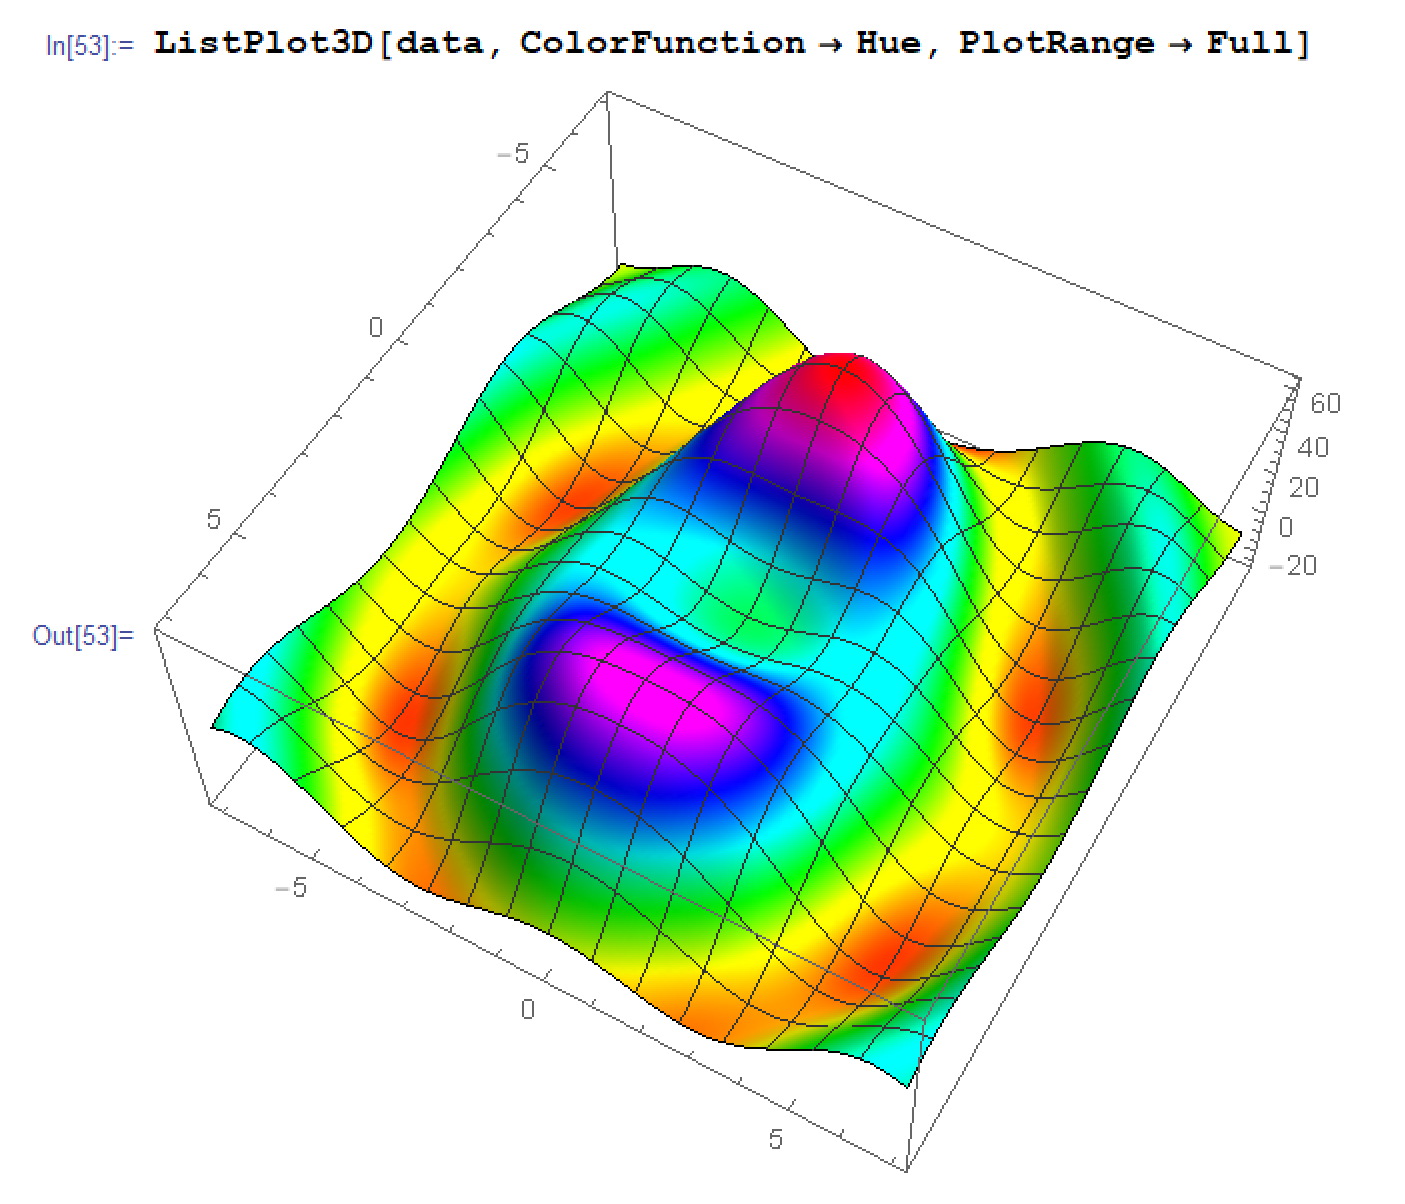
\includegraphics[scale=0.3]{conv-6}
\end{figure}



































	
\end{document}